\documentclass[conference]{IEEEtran}
\usepackage{amsmath,amssymb,amsthm}
\usepackage{graphicx}
\usepackage{booktabs}
\usepackage{multirow}
\usepackage{url}
\usepackage{cite}
\usepackage[hidelinks]{hyperref}
\usepackage{amsfonts}
\newtheorem{theorem}{Theorem}
\newtheorem{lemma}{Lemma}
\newtheorem{proposition}{Proposition}
\newtheorem{corollary}{Corollary}
\newtheorem{assumption}{Assumption}
\theoremstyle{remark}
\newtheorem{remark}{Remark}
\newcommand{\apref}[1]{Appendix~\ref{#1}}
\newcommand{\NEbProblems}{48}
\newcommand{\NBendersMeanS}{0.513}
\newcommand{\NBendersMaxS}{11.9}
\newcommand{\NMilpMeanS}{1.77}
\newcommand{\NMilpMaxS}{4.73}
\newcommand{\NSpeedupMean}{3.46}
\newcommand{\NBendersOneIter}{47}
\newcommand{\NBendersPhasec}{1}
\newcommand{\NBendersCertified}{48}
\newcommand{\NBendersGapMax}{1e-09}
\newcommand{\NBigmErrN}{20}
\newcommand{\NBigmErrMax}{0.0635}
\newcommand{\NBigmErrMaxMw}{6.35}
\newcommand{\NBigmSuboptN}{1}
\newcommand{\NBigmErrHour}{16}
\newcommand{\NBigmErrLimit}{lower}
\newcommand{\NBendersVsMilpTrueMaxdiff}{0.00626}
\newcommand{\NDcWidthMeanMw}{643.7}
\newcommand{\NGencoParams}{1{,}077{,}891}
\newcommand{\NLoadMaeIid}{0.0275}
\newcommand{\NLoadMaeScreen}{0.0314}
\newcommand{\NLoadMaeUnseen}{0.0295}
\newcommand{\NLoadPjfScreen}{0.112}
\newcommand{\NVmErrScreen}{0.00448}
\newcommand{\NInsecureScreen}{0.275}
\newcommand{\NInsecureUnseen}{0.405}
\newcommand{\NGencoMs}{10.3}
\newcommand{\NAcMs}{0.289}
\newcommand{\NSpRlast}{0.225}
\newcommand{\NAucRlast}{0.641}
\newcommand{\NSpRho}{0.219}
\newcommand{\NAucRho}{0.637}
\newcommand{\NSpRfirst}{0.224}
\newcommand{\NOodAucRlast}{0.586}
\newcommand{\NOodAucRho}{0.588}
\newcommand{\NRlastMedSeen}{0.0147}
\newcommand{\NRlastMedUnseen}{0.0158}
\newcommand{\NPtrMaeTest}{0.0136}
\newcommand{\NPtrMaeUnseen}{0.0184}
\newcommand{\NRawMaeTest}{0.0311}
\newcommand{\NRawMaeUnseen}{0.0295}
\newcommand{\NTrajOnlyMaeTest}{0.0197}
\newcommand{\NOutputsMaeTest}{0.0154}
\newcommand{\NLoadpredMaeTest}{0.0269}
\newcommand{\NPtrMaeRedPct}{56.3}
\newcommand{\NTrajOnlyMaeRedPct}{36.6}
\newcommand{\NClearPlainAab}{2.07}
\newcommand{\NFlagPlainAab}{98.4}
\newcommand{\NMissPlainAab}{0.07}
\newcommand{\NMissmaxPlainAab}{0.5}
\newcommand{\NClearNormalisedAab}{2.94}
\newcommand{\NFlagNormalisedAab}{97.8}
\newcommand{\NMissNormalisedAab}{0.04}
\newcommand{\NMissmaxNormalisedAab}{0.4}
\newcommand{\NClearPtrAab}{31.9}
\newcommand{\NFlagPtrAab}{77}
\newcommand{\NMissPtrAab}{0}
\newcommand{\NMissmaxPtrAab}{0}
\newcommand{\NClearPlainAaf}{4.67}
\newcommand{\NFlagPlainAaf}{96.3}
\newcommand{\NMissPlainAaf}{0.36}
\newcommand{\NMissmaxPlainAaf}{0.6}
\newcommand{\NClearNormalisedAaf}{8.28}
\newcommand{\NFlagNormalisedAaf}{93.7}
\newcommand{\NMissNormalisedAaf}{0.36}
\newcommand{\NMissmaxNormalisedAaf}{0.6}
\newcommand{\NClearPtrAaf}{54.4}
\newcommand{\NFlagPtrAaf}{60.7}
\newcommand{\NMissPtrAaf}{0.09}
\newcommand{\NMissmaxPtrAaf}{0.2}
\newcommand{\NClearPlainAb}{12.8}
\newcommand{\NFlagPlainAb}{90.1}
\newcommand{\NMissPlainAb}{0.695}
\newcommand{\NMissmaxPlainAb}{1.3}
\newcommand{\NClearNormalisedAb}{16.3}
\newcommand{\NFlagNormalisedAb}{87.7}
\newcommand{\NMissNormalisedAb}{0.53}
\newcommand{\NMissmaxNormalisedAb}{0.9}
\newcommand{\NClearPtrAb}{65.1}
\newcommand{\NFlagPtrAb}{52.7}
\newcommand{\NMissPtrAb}{0.305}
\newcommand{\NMissmaxPtrAb}{0.6}
\newcommand{\NClearUnseenPlainAab}{1.57}
\newcommand{\NFlagUnseenPlainAab}{99.1}
\newcommand{\NMissUnseenPlainAab}{0}
\newcommand{\NMissmaxUnseenPlainAab}{0}
\newcommand{\NClearUnseenNormalisedAab}{4.76}
\newcommand{\NFlagUnseenNormalisedAab}{97.2}
\newcommand{\NMissUnseenNormalisedAab}{0}
\newcommand{\NMissmaxUnseenNormalisedAab}{0}
\newcommand{\NClearUnseenPtrAab}{31.7}
\newcommand{\NFlagUnseenPtrAab}{81.1}
\newcommand{\NMissUnseenPtrAab}{0}
\newcommand{\NMissmaxUnseenPtrAab}{0}
\newcommand{\NClearUnseenPlainAaf}{5.77}
\newcommand{\NFlagUnseenPlainAaf}{96.6}
\newcommand{\NMissUnseenPlainAaf}{0}
\newcommand{\NMissmaxUnseenPlainAaf}{0}
\newcommand{\NClearUnseenNormalisedAaf}{5.32}
\newcommand{\NFlagUnseenNormalisedAaf}{96.8}
\newcommand{\NMissUnseenNormalisedAaf}{0}
\newcommand{\NMissmaxUnseenNormalisedAaf}{0}
\newcommand{\NClearUnseenPtrAaf}{55.8}
\newcommand{\NFlagUnseenPtrAaf}{66.7}
\newcommand{\NMissUnseenPtrAaf}{0.108}
\newcommand{\NMissmaxUnseenPtrAaf}{0.333}
\newcommand{\NClearUnseenPlainAb}{10.1}
\newcommand{\NFlagUnseenPlainAb}{94}
\newcommand{\NMissUnseenPlainAb}{0}
\newcommand{\NMissmaxUnseenPlainAb}{0}
\newcommand{\NClearUnseenNormalisedAb}{8.85}
\newcommand{\NFlagUnseenNormalisedAb}{94.7}
\newcommand{\NMissUnseenNormalisedAb}{0}
\newcommand{\NMissmaxUnseenNormalisedAb}{0}
\newcommand{\NClearUnseenPtrAb}{70.2}
\newcommand{\NFlagUnseenPtrAb}{57.9}
\newcommand{\NMissUnseenPtrAb}{0.367}
\newcommand{\NMissmaxUnseenPtrAb}{0.833}
\newcommand{\NTestN}{1{,}000}
\newcommand{\NTestInsecure}{266}
\newcommand{\NNSplits}{20}
\newcommand{\NEeLimits}{48}
\newcommand{\NEeChanged}{28}
\newcommand{\NEeShiftMaxMw}{279.0}
\newcommand{\NEeShiftMaxHour}{21}
\newcommand{\NEeShiftMaxLimit}{lower}
\newcommand{\NEeShiftMeanMw}{114.8}
\newcommand{\NEeWidthDcMeanMw}{643.7}
\newcommand{\NEeWidthAcMeanMw}{414.2}
\newcommand{\NEeWidthRedMeanPct}{42.5}
\newcommand{\NEeWidthRedMaxPct}{102.7}
\newcommand{\NEeEmptyHours}{1}
\newcommand{\NEeEmptyHourList}{18}
\newcommand{\NEeEmptyDcWidthMw}{270.6}
\newcommand{\NEeItersMean}{2.08}
\newcommand{\NEeItersMax}{3}
\newcommand{\NEeInfeasible}{0}
\newcommand{\NEeSecondsMean}{29.1}
\newcommand{\NItbDcBoundaryInsecure}{45}
\newcommand{\NItbN}{48}
\newcommand{\NItbMaxLoad}{1.14}
\newcommand{\NPoolTotal}{19{,}500}
\newcommand{\NFlaggedTotal}{12{,}699}
\newcommand{\NMissedTotal}{1}
\newcommand{\NGencoSTotal}{470.7}
\newcommand{\NExactAcSTotal}{3.41}
\newcommand{\NPoolClearedPct}{34.9}
\newcommand{\NItbDcBoundaryInsecurePct}{93.8}
\newcommand{\NAdvCases}{100}
\newcommand{\NAdvWins}{41}
\newcommand{\NAdvGainMax}{0.0117}
\newcommand{\NAdvGainMean}{-0.0076}
\newcommand{\NBessGainMeanMw}{561.8}
\newcommand{\NBessGainMinMw}{361.4}
\newcommand{\NBessGainMaxMw}{762.8}
\newcommand{\NBessFracMean}{0.777}
\newcommand{\NBessFracMin}{0.5}
\newcommand{\NWidthNobessMeanMw}{643.7}
\newcommand{\NBessAcInsecure}{35}
\newcommand{\NNobessAcInsecure}{39}
\newcommand{\NBessRows}{48}
\newcommand{\NLoadMaeIidPct}{2.75}
\newcommand{\NLoadMaeScreenPct}{3.14}
\newcommand{\NLoadMaeUnseenPct}{2.95}
\newcommand{\NLoadPjfScreenPct}{11.2}
\newcommand{\NInsecureScreenPct}{27.5}
\newcommand{\NInsecureUnseenPct}{40.5}
\newcommand{\NPtrMaeTestPct}{1.36}
\newcommand{\NPtrMaeUnseenPct}{1.84}
\newcommand{\NRawMaeTestPct}{3.11}
\newcommand{\NRawMaeUnseenPct}{2.95}
\newcommand{\NTrajOnlyMaeTestPct}{1.97}
\newcommand{\NOutputsMaeTestPct}{1.54}
\newcommand{\NLoadpredMaeTestPct}{2.69}
\newcommand{\NItbMaxLoadPct}{114.3}
\newcommand{\NAdvGainMaxPct}{1.17}
\newcommand{\NAdvGainMeanPct}{-0.76}


\begin{document}
\sloppy
\title{Certified AC Robust Secure Sets with GENCO in the Loop:\\
Benders Bounds, Physics-Trajectory Recalibration and Conformal Screening}

\author{\IEEEauthorblockN{Muhammad Abdillah}
\IEEEauthorblockA{Department of Electrical Engineering, Universitas Pertamina, Jakarta, Indonesia\\
muhammad.abdillah@universitaspertamina.ac.id}}
\maketitle

\begin{abstract}
The robust secure set (RSS) gives, for each hour, the range of dispatch that stays
secure for every PV and load realisation in a forecast box and in selected
contingencies. Its bilevel formulation was solved in the author's dissertation with DC
power flow and a big-M KKT MILP. We make the DC solution certified and then make it
AC-aware with the GENCO grid foundation model. (i) A two-phase combinatorial Benders
decomposition solves all \NEbProblems\ hourly problems of the IEEE 118-bus study to
certified optimality and shows that the big-M MILP misreports \NBigmErrN\ of them by up
to \NBigmErrMaxMw\,MW. (ii) Exact AC power flow shows that \NItbDcBoundaryInsecure\ of
\NItbN\ certified DC limits are AC-insecure; a GENCO-in-the-loop loop with exact AC
verification and correction cuts removes the violations; DC overstates the secure range
by \NEeWidthRedMeanPct\,\% on average and, in hour \NEeEmptyHourList, reports
\NEeEmptyDcWidthMw\,MW where the corrected set is empty. (iii) We show that the AC mismatch GENCO measures inside its
corrective layers explains \NPtrMaeRedPct\,\% of its own error (physics-trajectory
recalibration, PTR); wrapped in split-conformal screening it clears \NClearPtrAaf\,\% of
the secure scenarios without exact AC (\NClearPlainAaf\,\% for plain conformal), with a
finite-sample bound of 5\,\% on missed insecure scenarios (observed \NMissPtrAaf\,\%),
also in a topology GENCO never saw. Everything runs from one command with
\texttt{gridfm-graphkit} and \texttt{gridfm-datakit}.
\end{abstract}

\section{Introduction}
A robust secure set (RSS) tells the operator, for every hour, how far the dispatch of
controllable units can move while \emph{any} realisation of PV output and load inside a
forecast box remains secure in the base case and selected contingencies. Computing it is
a bilevel problem: nature chooses the worst PV/load vertex, the operator answers with the
best dispatch~\cite{abdillah2017thesis,yorino2018}. Two approximations made it tractable in the
first author's dissertation: DC power flow (thermal limits on MW instead of MVA, no
losses, no voltages) and a big-M KKT reformulation solved as one MILP.

This entry asks what a grid foundation model adds to such a \emph{certified} workflow.
GENCO~\cite{genco2026} is a unified neural solver for power flow, OPF and state
estimation trained with \texttt{gridfm-graphkit} on data from
\texttt{gridfm-datakit}~\cite{datakit2025}. We keep certification where it can be had
and use GENCO where it is strong: batched, differentiable AC prediction with an
internal physics check. Contributions:
\begin{enumerate}
\item A two-phase Benders decomposition for the RSS bilevel that needs no big-M on the
  primal side and returns a certified bound (Theorem~\ref{thm:main-benders}); on all 48 hourly
  problems it reproduces the true optimum and exposes reporting errors of the big-M MILP.
\item A GENCO-in-the-loop AC correction: GENCO screens pools of worst-case PV/load
  vertices in three topologies, exact AC verifies flagged ones, and AC-correction cuts
  are fed back to the Benders master.
\item \emph{Physics-trajectory recalibration} (PTR): the AC power mismatch that GENCO
  measures in each of its corrective layers explains a large part of its own error; a
  small recalibrator on that trajectory, wrapped in split-conformal screening, gives a
  finite-sample bound on missed insecure scenarios (Theorem~\ref{thm:main-conf}) while
  clearing many more secure scenarios than plain conformal screening, also in a topology
  GENCO never saw.
\item A GENCO-gradient adversary over the PV/load box, evaluated against exact AC power
  flow.
\end{enumerate}
The complete model (every equation used by the code) and complete proofs of all
statements are given in Appendices~A--G. Everything is reproducible with one command;
no result in this paper is set by hand.

\section{Robust Secure Set and Its Certified DC Solution}
\label{sec:rss}
\subsection{Bilevel model}
For hour $h$, nature chooses the PV and load vector $p=[P_R;P_D]$ in the box
$\mathcal P_h=[\underline p,\overline p]$ of (\ref{eq:box}) and the operator answers with the
dispatch $u\ge0$ of the dispatchable units. The DC line limits in the base topology and
in the two contingencies (\ref{eq:line}), the lossless balance (\ref{eq:bal}) and the
ramp-limited unit bounds (\ref{eq:ramp}) are stacked as $Ap+Bu\le b$ (\ref{eq:Abb}), and
$\mathcal U(p)=\{u\ge0:Bu\le b-Ap\}$. With the RSS index $\alpha=d^\top u$ (total output of
the non-balancing units), the RSS limits are~\cite{abdillah2017thesis,yorino2018}
\begin{equation}
\overline\alpha_h=\min_{p\in\mathcal P_h}\max_{u\in\mathcal U(p)}d^\top u,\qquad
\underline\alpha_h=\max_{p\in\mathcal P_h}\min_{u\in\mathcal U(p)}d^\top u .
\label{eq:rss}
\end{equation}
Theorem~\ref{thm:rss} (Appendix~\ref{app:dc}) proves that $[\underline\alpha_h,\overline\alpha_h]$ is
\emph{exactly} the set of index values that can be achieved for every realisation in the
box, so the set is empty iff $\underline\alpha_h>\overline\alpha_h$; Lemma~\ref{lem:vertex} proves
that both worst cases sit at vertices of the box. Both limits are linear bilevel programs
(\ref{eq:bilevel}) with an LP follower. The dissertation code solved them as one MILP after
replacing the follower by its KKT conditions linearised with $L=5\cdot10^4$
(\ref{eq:bigm}); Remark~\ref{rem:bigm} explains why that MILP can report values it does
not attain.

\subsection{Two-phase Benders decomposition}
\emph{Master (phase 1)}, (\ref{eq:mp-obj})--(\ref{eq:M6}): $p$, $u$ and binaries
$z=(z^u,z^\lambda)$ encoding the complementarity pattern,
\begin{equation}
u_k\le\overline U_kz^u_k,\qquad b_i-A_ip-B_iu\le S_i(1-z^\lambda_i),
\label{eq:mp-short}
\end{equation}
where $\overline U$ and $S_i=b_i-\min_{p,u}(A_ip+B_iu)$ (\ref{eq:S}) are \emph{exact} bounds
from the data: no dual variables and no arbitrary big-M. \emph{Subproblem:} is the dual
system $\mathrm{DF}(J_u,J_\ell)$ (\ref{eq:DF}) feasible for the pattern of the master point?
If yes, the point is bilevel optimal; if not, a Farkas certificate (Lemma~\ref{lem:farkas})
gives the combinatorial cut~\cite{codato2006}
\begin{equation}
\textstyle\sum_{k\in C_u}(1-z^u_k)+\sum_{i\in C_\ell}z^\lambda_i\ge1 .
\label{eq:cut-short}
\end{equation}
\emph{Robust value-function cut:} $d_2^\top u\ge\varphi_R$, where the static LP
(\ref{eq:phiR}) lets only the balancing unit adapt to $p$ (Lemma~\ref{lem:robust} proves
$\max_{\mathcal U(p)}d_2^\top u\ge\varphi_R$ for all $p$); its dual gives the first incumbent.
\emph{Phase 2:} if $\varphi_R$ does not exist or phase~1 exceeds 15 iterations, the duals
are lifted into the master with a bound on the dual side only (\ref{eq:lift}).

\begin{theorem}[Certificate; Theorems~\ref{thm:relax}--\ref{thm:phase2}]\label{thm:main-benders}
At every iteration $F(\hat p)\le\mathrm{OPT}\le\mathrm{UB}$: the incumbent is the exact
follower reaction at its $p$ (always attained) and the master value is a valid bound.
Phase~1 terminates finitely; at termination by dual feasibility the solution is
optimal. Phase~2 is exact if the dual bound $L_d$ is at least the uniform constant $L^\ast$
of Lemma~\ref{lem:dualbound}.
\end{theorem}

\section{GENCO in the Loop}
\label{sec:genco}
\subsection{AC-correction loop}
For every hour and limit, starting from the certified DC solution: (i) build a pool of
PV/load vertices (the Benders worst case, 60 random vertices and GENCO-gradient
vertices) and the DC follower response $u(p)$ for each, in all three topologies;
(ii) GENCO predicts the security quantities (\ref{eq:q}) of the whole pool in one batch;
(iii) the conformal rule (\ref{eq:flag}) flags scenarios; (iv) flagged scenarios are solved
with exact AC power flow (\ref{eq:acp})--(\ref{eq:acq}); (v) each verified overload derates
the DC limit of that branch and topology and AC losses tighten the slack bound
(\ref{eq:derate}); Benders is re-solved. Proposition~\ref{prop:nest} proves that the
corrected intervals are nested inside the DC interval, Corollary~\ref{cor:empty} that an
empty corrected set stays empty when the cuts of both limits are merged, and
Proposition~\ref{prop:loop} states what the output certifies.

\subsection{Probing the corrective layers}
GENCO's \texttt{GNS\_heterogeneous} evaluates, inside each of its $K$ corrective layers,
the AC mismatch of its intermediate estimate and feeds it back into the bus embeddings.
A forward hook on its residual layer records, at no extra cost,
\begin{equation}
\bar r^{(l)}=\frac1{|\mathcal N|}\sum_i\sqrt{(\Delta P^{(l)}_i)^2+(\Delta Q^{(l)}_i)^2},\qquad
\rho=\frac{\bar r^{(K)}}{\bar r^{(1)}} .
\label{eq:traj-short}
\end{equation}

\subsection{Physics-trajectory recalibration (PTR) and conformal screening}
For each security quantity $q_k$ with limit $\ell_k$ and GENCO prediction $\hat q_k$, PTR
fits on a \emph{tune} split a regressor of GENCO's error on GENCO-internal features
$z=(\hat q,\bar r^{(1)},\dots,\bar r^{(K)},\rho)$ (\ref{eq:ptr}) and sets
$\tilde q_k=\hat q_k+g_k(z)$. On an independent \emph{calibration} split~\cite{lei2018} of
size $n$ the scores $s_k=q_k-\tilde q_k$ give the threshold
\begin{equation}
\begin{aligned}
c_k&=\text{the }\lceil(n+1)(1-\alpha/3)\rceil\text{-th smallest score},\\
\text{clear}&\iff\tilde q_k+c_k\le\ell_k\quad\forall k .
\end{aligned}
\label{eq:conf-short}
\end{equation}
\begin{theorem}[No-miss guarantee; Theorem~\ref{thm:conf}]\label{thm:main-conf}
For a test scenario exchangeable with the calibration scenarios and any $g_k$ fitted
without them, $\Pr[\text{insecure and cleared}]\le\alpha$.
\end{theorem}
The proof (Appendix~\ref{app:conf}) uses the split-conformal quantile Lemma~\ref{lem:conf}
and a union bound over the three quantities. $g_k\equiv0$ is plain split-conformal; we
also compare a residual-normalised score $(q_k-\hat q_k)/(\sigma_k+\beta_k\bar r^{(K)})$. PTR
uses no hour or topology label, so it applies unchanged to a topology GENCO never saw
(where, however, exchangeability is not guaranteed).

\subsection{Gradient adversary}
GENCO is differentiable in its inputs. With the dispatch fixed, we ascend the smooth
maximum (\ref{eq:J}) of GENCO-predicted loading over the three topologies by projected
sign-gradient steps (\ref{eq:adv}) in $\mathcal P_h$ (Lemma~\ref{lem:lse} bounds the
smoothing error by $\tau\log|\mathcal E|$), round to the nearest vertex, recompute $u(p)$ and
add the point to the pool, where it is verified exactly.

\section{Test System and Implementation}
\label{sec:setup}
\textbf{Grid.} PGLib-OPF v23.07 IEEE 118-bus case~\cite{pglib} (19 dispatchable units, 35 synchronous
condensers, 186 branches with MVA ratings). 20 PV buses grouped in five sites, hourly
load and PV profile, PV error $0.3\,h/24$ of capacity and load error $0.03\,h/24$, PV only
in hours 7--18, ramp window $\pm30\,\%$ of capacity around a DC-OPF base dispatch, and
the contingencies of the dissertation (one circuit of 69--70 and of 100--103 lost).
Generator voltage set-points come from one AC-OPF per hour (pandapower~\cite{pandapower}) at the centre of
the box, as \texttt{gridfm-datakit} does with its OPF step.

\textbf{Exact AC.} \texttt{gridfm-datakit}~1.1.0 in PF mode with the
\texttt{lightsim2grid} Newton--Raphson solver; its Julia OPF step is replaced by our
operating-point source (the RSS dispatches). Security = branch apparent power within
rating in all three topologies, PQ-bus voltage within $[0.94,1.06]$ p.u.\ (0.01 p.u.\
tolerance; the largest over-voltage in all data is 0.0055 p.u.), slack within capacity.
Generator reactive limits are not enforced by the PF and are reported only.

\textbf{GENCO.} The official checkpoints (\texttt{gridfm/genco-pf-datakit}) could not be
downloaded from our compute environment, so we trained the GENCO architecture
(\texttt{GNS\_heterogeneous}, PowerFlow task, layered physics loss) from scratch with
\texttt{gridfm-graphkit}~0.9.0.3 on 24{,}000 datakit scenarios of the RSS operating
region (all hours, three topologies, vertex and interior PV/load, vertex and interior
dispatches), in a small CPU configuration ($K=10$ layers, hidden size 24, 4 heads,
\NGencoParams\ parameters, 15 epochs, about 4\,h on two CPU cores). The code loads an
official checkpoint unchanged when it is available.

\textbf{Data for evaluation} (all exact AC, never used for training): 2{,}000 draws of
the training distribution; 3{,}000 draws of the \emph{screening distribution} (DC
follower responses at Benders worst-case or random vertices, random line derating
$[0.85,1]$, random topology), split 1{,}000/1{,}000/1{,}000 into tune, calibration and
test; and 600 screening draws in a topology GENCO never saw (one circuit of 49--66 lost).
All timings: one 2-core CPU, no GPU.

\section{Results}
\label{sec:results}
Every number below is read from \texttt{results/} by \texttt{experiments/e7\_numbers.py}.

\subsection{Certified DC robust secure set (E1)}
All \NEbProblems\ bilevel problems (24 hours, upper and lower limit) were solved to
certified optimality (master bound equals the attained value to $10^{-9}$). In
\NBendersOneIter\ of them the robust value-function cut is tight and Benders stops after
one master solve; one problem (hour 21, upper) needed phase~2. Mean time is
\NBendersMeanS\,s against \NMilpMeanS\,s for the big-M MILP of the dissertation code
(both with HiGHS on the same CPU), but the more important difference is correctness
(Fig.~\ref{fig:dc}b): the MILP's reported objective differs from the value its own
leader decision attains in \NBigmErrN\ of \NEbProblems\ problems, by up to
\NBigmErrMaxMw\,MW (hour \NBigmErrHour, \NBigmErrLimit\ limit), and in
\NBigmSuboptN\ problem its leader decision is not optimal. This is the known failure
mode of a fixed big-M in bilevel KKT reformulations~\cite{pineda2019bigm}; the Benders
certificate removes it. The mean DC secure range is \NDcWidthMeanMw\,MW.

\begin{figure*}[t]
\centering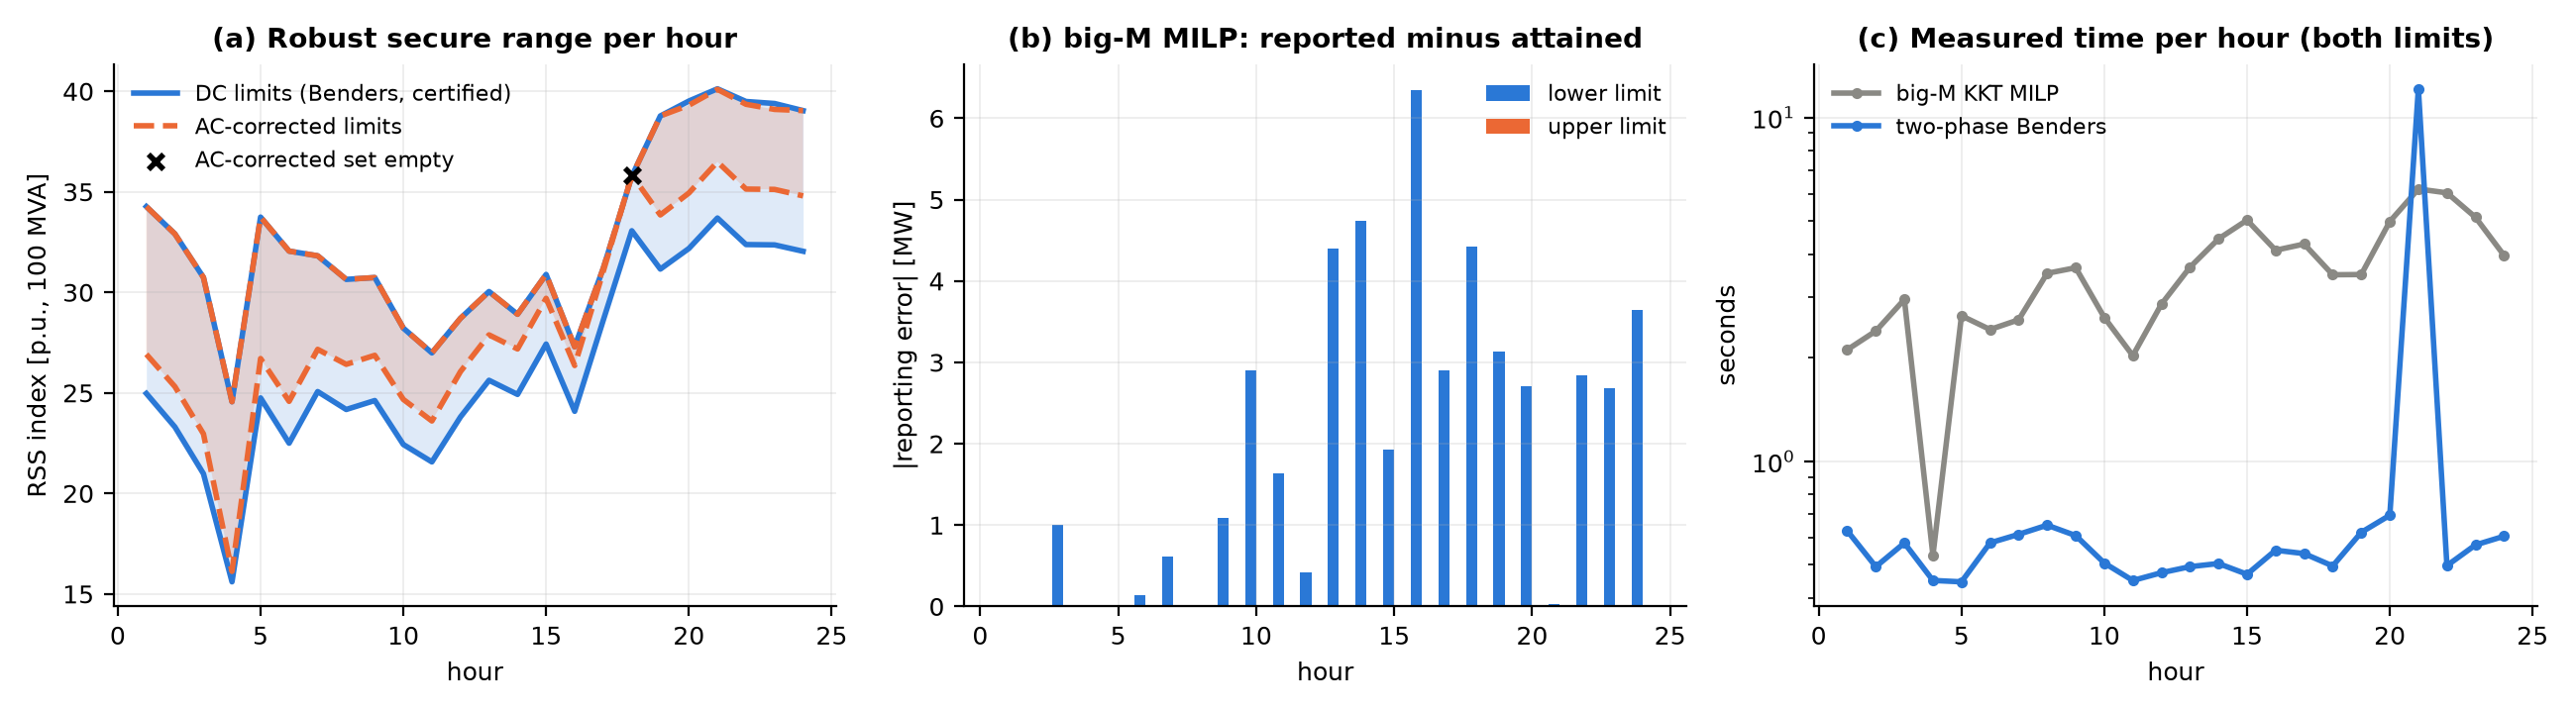
\includegraphics[width=\textwidth]{../results/figures/fig1_dc_rss.png}
\caption{(a) Certified DC limits per hour and AC-corrected limits from the GENCO-in-the-loop
correction (E4). (b) Big-M MILP: reported objective minus value attained by its leader
decision. (c) Measured solve time.}
\label{fig:dc}
\end{figure*}

\subsection{GENCO accuracy and its corrective-layer trajectory (E3)}
The trained GENCO (\NGencoParams\ parameters) predicts the maximum branch loading
with mean absolute error \NLoadMaeIidPct\,\% (training distribution),
\NLoadMaeScreenPct\,\% (screening distribution) and \NLoadMaeUnseenPct\,\% (unseen
topology) of the rating, and
voltage magnitudes with mean worst-bus error \NVmErrScreen\,p.u. The error is
\emph{not} uniform (Fig.~\ref{fig:probe}a): GENCO under-predicts a cluster of
contingency-100--103 scenarios. Inside GENCO the AC mismatch contracts by more than two
orders of magnitude over the $K=10$ layers, and almost identically in the unseen
topology (Fig.~\ref{fig:probe}b). Single scalars of that trajectory are weak error
indicators (Spearman \NSpRlast\ for $\bar r^{(K)}$, AUROC \NAucRlast\ for the 10\,\%
largest errors, \NOodAucRlast\ for detecting the unseen topology). The \emph{whole}
trajectory is informative (Fig.~\ref{fig:probe}c): a recalibrator that sees only
$\bar r^{(1)},\dots,\bar r^{(K)},\rho$ removes \NTrajOnlyMaeRedPct\,\% of the error, and PTR
(trajectory plus GENCO outputs) removes \NPtrMaeRedPct\,\% (MAE \NRawMaeTestPct\,\%
$\to$ \NPtrMaeTestPct\,\%) and reduces it in the unseen topology from
\NRawMaeUnseenPct\,\% to \NPtrMaeUnseenPct\,\%.

\begin{figure*}[t]
\centering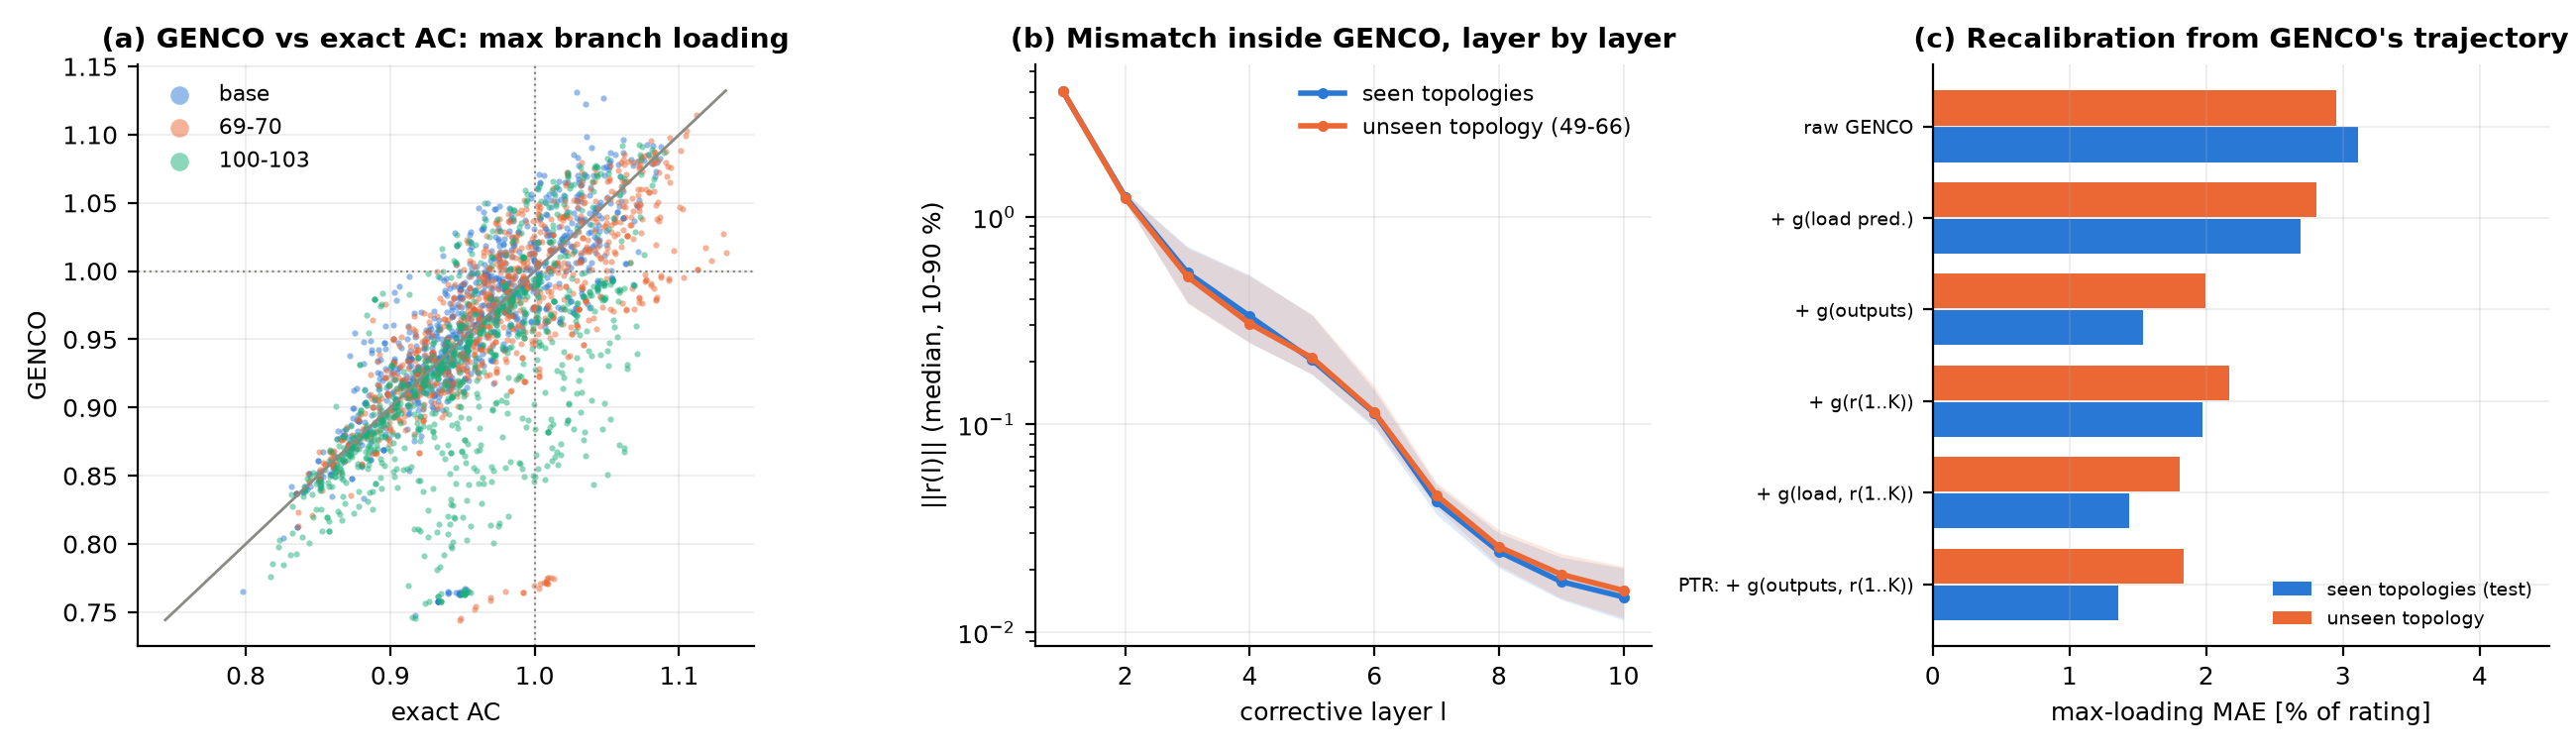
\includegraphics[width=\textwidth]{../results/figures/fig2_genco_probe.png}
\caption{(a) GENCO vs.\ exact AC (screening test set), by topology. (b) AC mismatch
measured inside GENCO, layer by layer. (c) Ablation: what the recalibrator sees vs.\
remaining error (fitted on the tune split, evaluated on test and unseen topology).}
\label{fig:probe}
\end{figure*}

\subsection{Screening with a guarantee (E3)}
Table~\ref{tab:conf} and Fig.~\ref{fig:conf} report the screening over \NNSplits\ random
tune/calibration/test splits of the 3{,}000 screening scenarios (\NTestInsecure\ of
\NTestN\ test scenarios are insecure: the screening distribution sits on the RSS
boundary by construction). At $\alpha=0.05$, plain split-conformal screening can clear
only \NClearPlainAaf\,\% of the secure scenarios, because GENCO's error tail forces a wide
margin; PTR clears \NClearPtrAaf\,\% in seen topologies and \NClearUnseenPtrAaf\,\% in
the unseen one. The observed rate of insecure-and-cleared scenarios is
\NMissPtrAaf\,\% (worst split \NMissmaxPtrAaf\,\%), far below the 5\,\% guarantee.

\begin{table}[t]
\centering
\caption{Secure scenarios cleared without exact AC [\%] and observed miss rate [\%]
(mean of \NNSplits\ splits; miss = insecure and cleared).}
\label{tab:conf}
\setlength{\tabcolsep}{3.5pt}
\begin{tabular}{@{}llccc@{}}
\toprule
 & & $\alpha=0.01$ & $\alpha=0.05$ & $\alpha=0.10$\\
\midrule
\multirow{3}{*}{\shortstack[l]{seen\\topol.}}
 & plain      & \NClearPlainAab & \NClearPlainAaf & \NClearPlainAb\\
 & normalised & \NClearNormalisedAab & \NClearNormalisedAaf & \NClearNormalisedAb\\
 & PTR        & \textbf{\NClearPtrAab} & \textbf{\NClearPtrAaf} & \textbf{\NClearPtrAb}\\
 & PTR miss   & \NMissPtrAab & \NMissPtrAaf & \NMissPtrAb\\
\midrule
\multirow{3}{*}{\shortstack[l]{unseen\\49--66}}
 & plain      & \NClearUnseenPlainAab & \NClearUnseenPlainAaf & \NClearUnseenPlainAb\\
 & normalised & \NClearUnseenNormalisedAab & \NClearUnseenNormalisedAaf & \NClearUnseenNormalisedAb\\
 & PTR        & \textbf{\NClearUnseenPtrAab} & \textbf{\NClearUnseenPtrAaf} & \textbf{\NClearUnseenPtrAb}\\
 & PTR miss   & \NMissUnseenPtrAab & \NMissUnseenPtrAaf & \NMissUnseenPtrAb\\
\bottomrule
\end{tabular}
\end{table}

\begin{figure*}[t]
\centering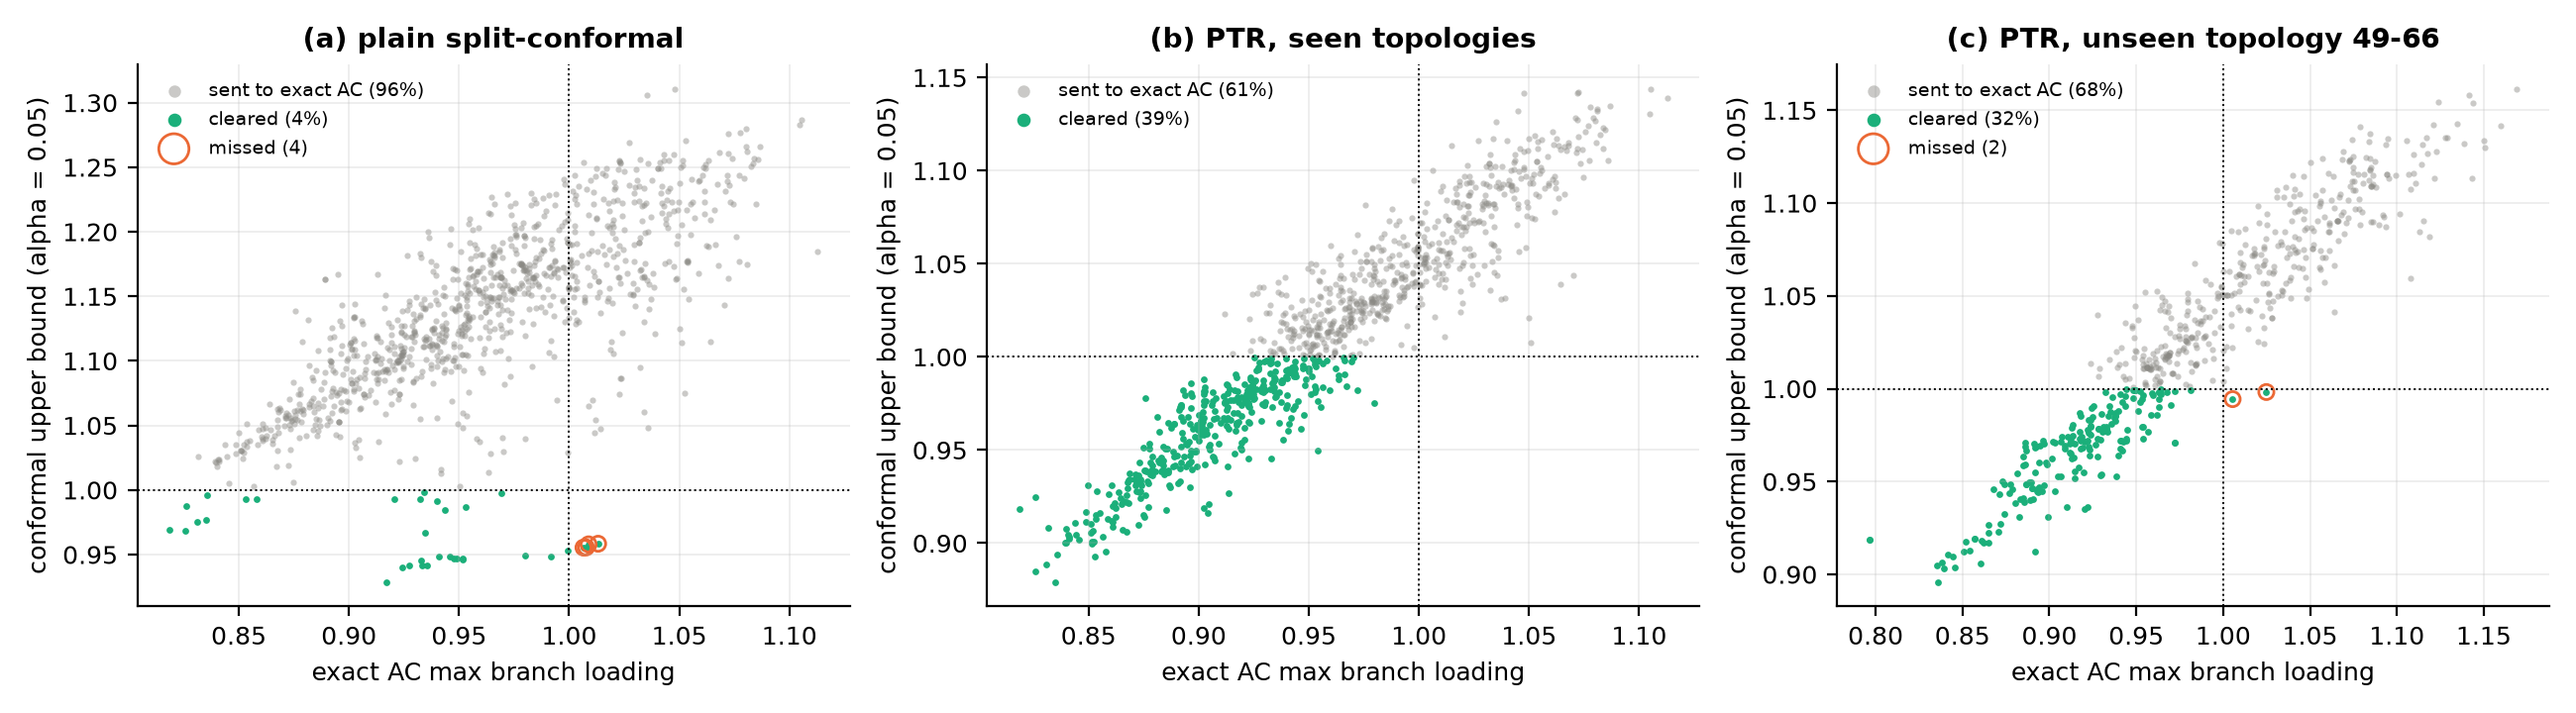
\includegraphics[width=\textwidth]{../results/figures/fig6_screen.png}
\caption{Conformal upper bound on the maximum branch loading vs.\ exact AC at $\alpha=0.05$
(one split). Green: cleared without exact AC. Plain conformal must place almost all
scenarios above 1; PTR clears most secure ones, also in the unseen topology.}
\label{fig:conf}
\end{figure*}

\subsection{AC-corrected robust secure set (E4)}
In \NItbDcBoundaryInsecure\ of \NItbN\ hour-limit problems the certified DC limit is
\emph{not} AC-secure: some vertex of the PV/load box overloads a branch in AC (worst
loading \NItbMaxLoadPct\,\% of rating). The GENCO-in-the-loop correction removes all verified
violations in at most \NEeItersMax\ iterations (\NEeSecondsMean\,s per limit on
average). It moves \NEeChanged\ of \NEeLimits\ limits, by up to \NEeShiftMaxMw\,MW
(hour \NEeShiftMaxHour, \NEeShiftMaxLimit\ limit), and the mean secure range shrinks from
\NEeWidthDcMeanMw\ to \NEeWidthAcMeanMw\,MW (Fig.~\ref{fig:dc}a, Fig.~\ref{fig:ac}a): DC
overstates the range by \NEeWidthRedMeanPct\,\% on average. In hour \NEeEmptyHourList\
the corrected lower limit exceeds the upper one, i.e.\ the corrected model admits no
robust secure dispatch although DC reports a range of \NEeEmptyDcWidthMw\,MW. Over the whole run, PTR
cleared \NPoolClearedPct\,\% of the \NPoolTotal\ pool scenarios (the pools sit on the
boundary, so this is lower than in E3); an audit that solved every pool scenario exactly
found \NMissedTotal\ insecure scenario among the cleared ones (first iteration of one
problem; none in any final iteration). The GENCO-gradient adversary found a vertex worse
than all Benders and random vertices in \NAdvWins\ of \NAdvCases\ searches, by at most
\NAdvGainMaxPct\,\% of rating (Fig.~\ref{fig:ac}b); the DC worst-case vertex is usually already
close to the AC worst case.

\begin{figure*}[t]
\centering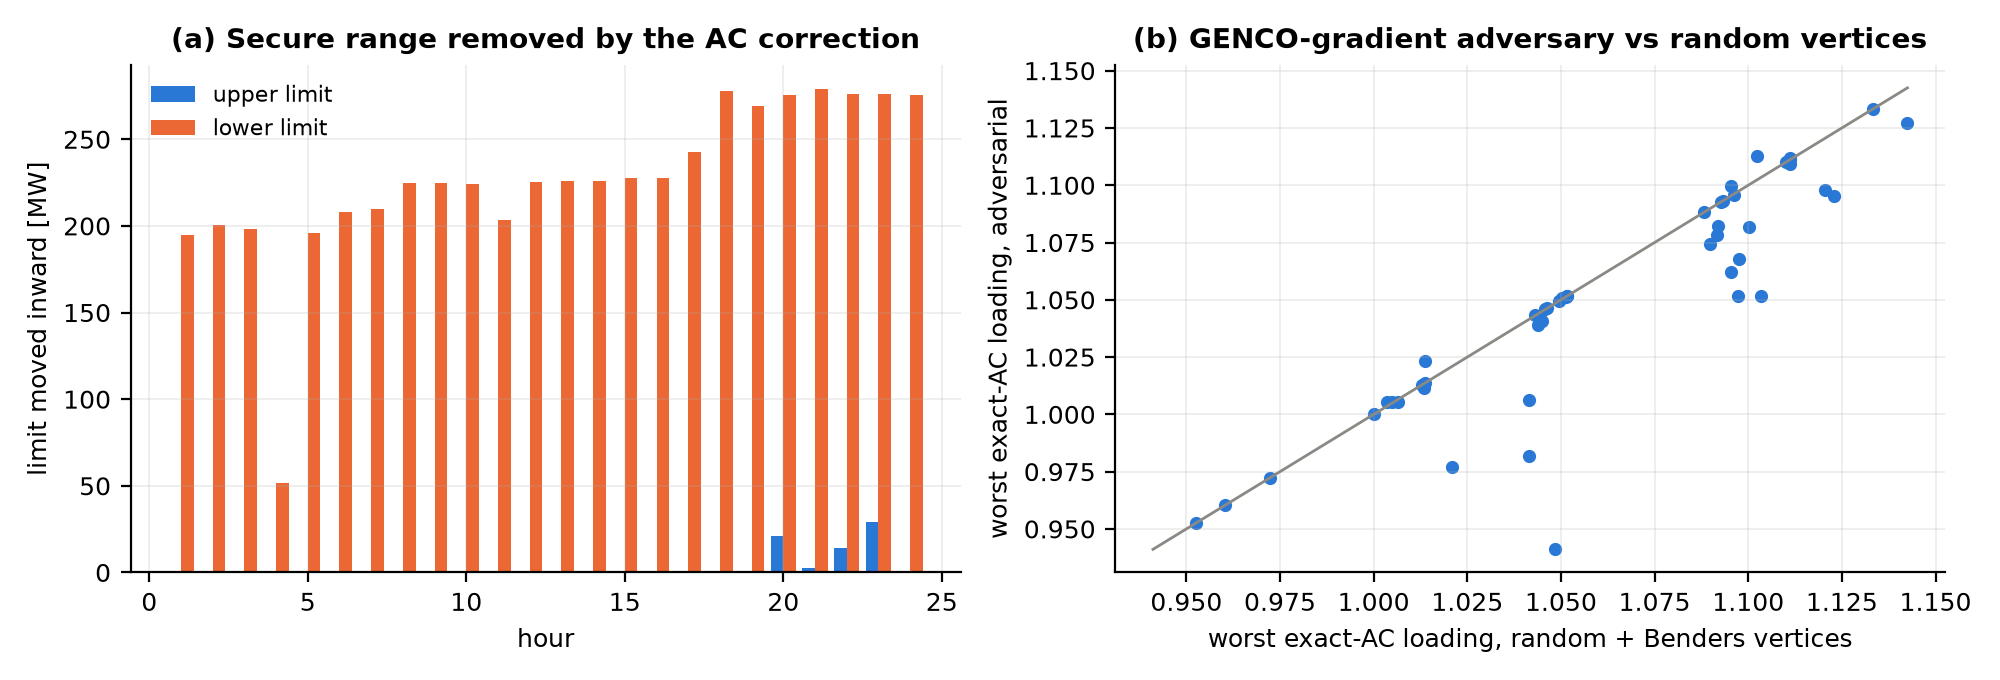
\includegraphics[width=0.78\textwidth]{../results/figures/fig4_ac_loop.png}
\caption{(a) Secure range removed by the AC correction, per hour and limit (MW the limit
moved inward). (b) Worst exact-AC loading at GENCO-adversarial vs.\ Benders/random
vertices (one point per search).}
\label{fig:ac}
\end{figure*}

\subsection{Extension: second-life EV batteries (E5)}
Placing second-life EV batteries ($P=\mathrm{SoH}\cdot0.35\cdot$ PV capacity, 20 sites,
3.6\,p.u.\ in total) as follower resources widens the certified DC range by
\NBessGainMeanMw\,MW on average (\NBessGainMinMw--\NBessGainMaxMw), i.e.\ \NBessFracMean\
of the theoretical $2P_\mathrm{bess}$. The worst-case points are AC-insecure in
\NBessAcInsecure\ of \NBessRows\ cases with batteries and \NNobessAcInsecure\ of 48
without, so the AC correction of E4 is needed with batteries too.


\section{Discussion and Limitations}
\textbf{Where GENCO helps.} On a 118-bus case on CPU, the Newton--Raphson solver of
\texttt{lightsim2grid} needs \NAcMs\,ms per scenario and our GENCO \NGencoMs\,ms, so
GENCO is \emph{not} a speed-up here; we do not claim one. What GENCO adds is (a) a
differentiable surrogate over the uncertainty box, (b) a batched prediction with a
self-measured physics trajectory, which PTR turns into the share of exact checks that
can be skipped with a guarantee. That share, not raw inference time, is what transfers
to settings where the exact check is expensive (larger grids, AC-OPF re-dispatch,
reactive limits, many contingencies, GPU batches).

\textbf{What is certified.} The DC bound is certified (Theorem~\ref{thm:main-benders}). The
AC-corrected limit is certified for the corrected DC model, and every pool scenario is
AC-secure exactly (flagged) or with probability $1-\alpha$ (cleared). This is not a
certificate over the continuous box in AC; an exact AC robust counterpart remains open.
The correction derates active-power limits; all lower-limit problems reached the 0.8
derating floor on some branch, a sign that the MVA overload there is partly reactive, so
the corrected limits are conservative (the empty set of hour \NEeEmptyHourList\ is a
statement about the corrected model, not a proof that no AC-secure dispatch exists).

\textbf{Honest limitations.} The official GENCO checkpoints could not be downloaded from
our environment, so a small GENCO was trained from scratch on CPU; a larger model will
change all GENCO numbers (the code loads official weights unchanged). Generator
reactive limits are not enforced by the power flow. The conformal guarantee needs
exchangeability between calibration and use; the unseen-topology results are an
empirical check of robustness, not a guarantee. The adversary improved on the Benders and random
vertices in \NAdvWins\ of \NAdvCases\ searches, with small gains.

\section{Conclusion}
A certified Benders bound, exact AC where it matters, and GENCO with
physics-trajectory recalibration where a guarantee allows skipping exact AC together
turn the DC robust secure set of the dissertation into an AC-aware one, and expose
errors of the big-M MILP on the way. Code, data generation, trained weights, results
and an interactive Space are open.

\clearpage\onecolumn\setlength{\vsize}{\textheight}% full-height one-column appendix pages
\raggedbottom
\allowdisplaybreaks
\appendices
% =====================================================================
% Complete formulation and proofs. Included as the appendix of main.tex
% and as the body of supplement.tex. Every equation matches the code in
% genco_rss/ (file and function given in brackets).
% =====================================================================

\section{DC Model of the Robust Secure Set}
\label{app:dc}

\subsection{Sets, data and decision variables}
Buses $\mathcal N$ ($|\mathcal N|=118$) with reference bus $n_0$; branches $\mathcal L$
($|\mathcal L|=186$) with reactance $x_\ell$ and MVA rating $r_\ell$ (p.u., base 100\,MVA);
dispatchable units $\mathcal G$ ($|\mathcal G|=19$) with the balancing (slack) unit
$g_0\in\mathcal G$ located at $n_0$; PV buses $\mathcal R$ ($|\mathcal R|=20$); load buses
$\mathcal D$; topologies $s\in\mathcal S=\{0,1,2\}$ (base case; one circuit of 69--70 lost;
one circuit of 100--103 lost). Incidence matrices $C_G\in\{0,1\}^{|\mathcal N|\times|\mathcal G|}$,
$C_R$, $C_D$ map units, PV injections and loads to buses.

Uncertain vector (nature) $p=[P_R;P_D]\in\mathbb R^{n_p}$, $n_p=|\mathcal R|+|\mathcal D|$.
Dispatch (operator) $u\in\mathbb R^{n_u}_{\ge 0}$, $n_u=|\mathcal G|$
(plus $2|\mathcal R|$ battery variables in \apref{app:bess}).

\subsection{Power transfer distribution factors}
[\texttt{grid.ptdf}] Let $C\in\{-1,0,1\}^{|\mathcal L|\times|\mathcal N|}$ be the
branch--bus incidence matrix and $X_s=\mathrm{diag}(x^s_\ell)$ with
\begin{equation}
x^s_\ell=\begin{cases}2x_\ell & \ell \text{ is the corridor of } s\ (\text{one of two identical parallel circuits lost}),\\
x_\ell & \text{otherwise,}\end{cases}
\label{eq:xs}
\end{equation}
since two identical circuits in parallel have half the reactance of one. As in the
dissertation data, the corridor rating is kept.
With $B_f^s=X_s^{-1}C$, $B_{\rm bus}^s=C^\top X_s^{-1}C$ and $\mathcal N'=\mathcal N\setminus\{n_0\}$,
\begin{equation}
H_s[:,\mathcal N']=B_f^s[:,\mathcal N']\big(B^s_{\rm bus}[\mathcal N',\mathcal N']\big)^{-1},\qquad H_s[:,n_0]=0 .
\label{eq:ptdf}
\end{equation}
The DC branch flows of an operating point in topology $s$ are
\begin{equation}
f_s(p,u)=H_s\big(C_Gu+C_RP_R-C_DP_D\big).
\label{eq:flow}
\end{equation}
Because the slack unit sits at $n_0$, column $H_sC_G[:,g_0]=0$: the slack unit does not
appear in any line constraint (used in Lemma~\ref{lem:robust}).

\subsection{Constraints}
[\texttt{grid.rss\_matrices}] For derating factors $\kappa_s\in(0,1]^{|\mathcal L|}$
($\kappa\equiv1$ in the DC study, \apref{app:ac} otherwise):
\begin{align}
&-\kappa_s\circ r\le f_s(p,u)\le\kappa_s\circ r, && s\in\mathcal S, \label{eq:line}\\
&\mathbf 1^\top u+\mathbf 1^\top P_R-\mathbf 1^\top P_D=0, && \text{(lossless balance)} \label{eq:bal}\\
&\underline u\le u\le\overline u. && \label{eq:genb}
\end{align}
[\texttt{grid.gen\_limits}, \texttt{rss.dc\_opf}] With $u^0$ the linear-cost DC-OPF dispatch at
the box centre and ramp fraction $\rho=0.3$:
\begin{equation}
\underline u_k=\max(P^{\min}_k,u^0_k-\rho P^{\max}_k),\quad
\overline u_k=\min(P^{\max}_k,u^0_k+\rho P^{\max}_k)\ (k\neq g_0),\quad
[\underline u_{g_0},\overline u_{g_0}]=[P^{\min}_{g_0},P^{\max}_{g_0}].
\label{eq:ramp}
\end{equation}
Stacking (\ref{eq:line})--(\ref{eq:genb}) row-wise gives the polyhedral system
\begin{equation}
Ap+Bu\le b,\qquad
A=\begin{bmatrix}A_\ell\\-A_\ell\\ a^\top\\-a^\top\\0\\0\end{bmatrix},\
B=\begin{bmatrix}B_\ell\\-B_\ell\\ \mathbf 1^\top\\-\mathbf 1^\top\\-I\\I\end{bmatrix},\
b=\begin{bmatrix}\kappa\circ r\\ \kappa\circ r\\0\\0\\-\underline u\\ \overline u\end{bmatrix},
\label{eq:Abb}
\end{equation}
with $A_\ell=[H_sC_R,\,-H_sC_D]_{s\in\mathcal S}$, $B_\ell=[H_sC_G]_{s\in\mathcal S}$
(stacked over $s$), $a=[\mathbf 1;-\mathbf 1]$. The follower's feasible set is
\begin{equation}
\mathcal U(p)=\{u\in\mathbb R^{n_u}_{\ge0}: Bu\le b-Ap\}.
\label{eq:U}
\end{equation}

\subsection{Uncertainty set}
[\texttt{grid.scenario\_box}] For hour $h$, with PV forecast $\hat P_{R}$, capacity
$\bar P_R$, forecast load $\hat P_D$, $e_{\rm PV}(h)=0.3\,h/24$ and $e_D(h)=0.03\,h/24$:
\begin{equation}
\mathcal P_h=\Big\{p:\ \big[\hat P_R-e_{\rm PV}\bar P_R\big]_0^{\bar P_R}\le P_R\le\big[\hat P_R+e_{\rm PV}\bar P_R\big]_0^{\bar P_R},\
(1-e_D)\hat P_D\le P_D\le(1+e_D)\hat P_D\Big\},
\label{eq:box}
\end{equation}
where $[\cdot]_0^{\bar P}$ clips to $[0,\bar P]$ and $P_R\equiv0$ for $h\notin[7,18]$.
$\mathcal P_h=[\underline p,\overline p]$ is a box with vertex set $V(\mathcal P_h)$.

\subsection{Robust secure set}
The RSS index is the total output of the non-balancing units,
\begin{equation}
\alpha=d^\top u,\qquad d_k=1\ (k\neq g_0),\ d_{g_0}=0 .
\label{eq:index}
\end{equation}
\begin{assumption}\label{as:feas}
$\mathcal U(p)\neq\emptyset$ for every $p\in\mathcal P_h$ (the follower can always serve the
load; checked by Benders, which otherwise reports infeasibility).
\end{assumption}
Define the follower value functions and the RSS limits
\begin{align}
\varphi(p)&=\max\{d^\top u:u\in\mathcal U(p)\}, & \psi(p)&=\min\{d^\top u:u\in\mathcal U(p)\},\label{eq:vf}\\
\overline\alpha_h&=\min_{p\in\mathcal P_h}\varphi(p), & \underline\alpha_h&=\max_{p\in\mathcal P_h}\psi(p). \label{eq:rssdef}
\end{align}

\begin{theorem}[Meaning of the RSS interval]\label{thm:rss}
Under Assumption~\ref{as:feas}, a value $\alpha$ is achievable for \emph{every}
realisation, i.e.\ $\forall p\in\mathcal P_h\ \exists u\in\mathcal U(p): d^\top u=\alpha$, if
and only if $\alpha\in[\underline\alpha_h,\overline\alpha_h]$. In particular the robust
secure set is empty if and only if $\underline\alpha_h>\overline\alpha_h$.
\end{theorem}
\begin{proof}
Fix $p$. $\mathcal U(p)$ is a non-empty polytope (bounded by (\ref{eq:genb})), hence
compact and convex; its image under the linear map $u\mapsto d^\top u$ is a compact
interval, which by (\ref{eq:vf}) equals $[\psi(p),\varphi(p)]$.
($\Leftarrow$) If $\underline\alpha_h\le\alpha\le\overline\alpha_h$, then for every $p$,
$\psi(p)\le\underline\alpha_h\le\alpha\le\overline\alpha_h\le\varphi(p)$, so $\alpha$ lies in the
image interval and some $u\in\mathcal U(p)$ attains it.
($\Rightarrow$) If $\alpha>\overline\alpha_h$, take $p^\star\in\arg\min\varphi$ (exists by
Lemma~\ref{lem:vertex}); then $\alpha>\varphi(p^\star)$ and no $u\in\mathcal U(p^\star)$ attains
$\alpha$. The case $\alpha<\underline\alpha_h$ is symmetric with $\arg\max\psi$.
\end{proof}

\begin{lemma}[Worst cases are vertices]\label{lem:vertex}
$\varphi$ is concave and $\psi$ is convex on $\mathcal P_h$. Hence
\[
\overline\alpha_h=\min_{p\in V(\mathcal P_h)}\varphi(p),\qquad
\underline\alpha_h=\max_{p\in V(\mathcal P_h)}\psi(p).
\]
\end{lemma}
\begin{proof}
Let $p_1,p_2\in\mathcal P_h$, $\theta\in[0,1]$, and $u_i\in\mathcal U(p_i)$ optimal for
$\varphi(p_i)$. Then $u_\theta=\theta u_1+(1-\theta)u_2\ge0$ and
$Bu_\theta=\theta Bu_1+(1-\theta)Bu_2\le b-A(\theta p_1+(1-\theta)p_2)$, so
$u_\theta\in\mathcal U(p_\theta)$ and $\varphi(p_\theta)\ge d^\top u_\theta=\theta\varphi(p_1)+(1-\theta)\varphi(p_2)$:
$\varphi$ is concave. The same argument with minimisers shows that $\psi$ is convex.
A concave function on a polytope attains its minimum at a vertex (write any point as a
convex combination of vertices and use concavity: $\varphi(\sum\theta_jv_j)\ge\sum\theta_j\varphi(v_j)\ge\min_j\varphi(v_j)$);
symmetrically a convex function attains its maximum at a vertex.
\end{proof}

\section{Bilevel Form, KKT Conditions and the Big-M Baseline}
\label{app:bilevel}
Both limits are instances of the linear bilevel program [\texttt{benders.solve}]
\begin{equation}
\mathrm{OPT}=\max_{p\in\mathcal P_h,\,u}\ c_1^\top p+d_1^\top u\quad\text{s.t.}\quad
u\in\arg\max_{v\in\mathcal U(p)} d_2^\top v,
\label{eq:bilevel}
\end{equation}
with $c_1=0$ and $(d_1,d_2)=(-d,d)$ for the upper limit ($\overline\alpha_h=-\mathrm{OPT}$) and
$(d_1,d_2)=(d,-d)$ for the lower limit ($\underline\alpha_h=\mathrm{OPT}$).
\begin{remark}\label{rem:optimistic}
Since $d_1=-d_2$, every follower optimum gives the leader the same value
$d_1^\top u=-\max_{v}d_2^\top v$; optimistic and pessimistic bilevel solutions coincide. For
general data we use the optimistic convention: the attained value at $p$ is
\begin{equation}
F(p)=c_1^\top p+\max\{d_1^\top u:\ u\in\mathcal U(p),\ d_2^\top u=\max_{v\in\mathcal U(p)}d_2^\top v\},
\label{eq:Fp}
\end{equation}
computed by two LPs [\texttt{benders.follower\_response}].
\end{remark}
\textbf{Follower dual and KKT.} The follower LP $\max\{d_2^\top u: Bu\le b-Ap,\ u\ge0\}$ has the dual
$\min\{\lambda^\top(b-Ap):\ B^\top\lambda\ge d_2,\ \lambda\ge0\}$. A feasible $u$ is optimal iff
there is $\lambda$ with
\begin{equation}
\lambda\ge0,\quad B^\top\lambda\ge d_2,\quad u_k\,(B^\top\lambda-d_2)_k=0\ \forall k,\quad
\lambda_i\,(b-Ap-Bu)_i=0\ \forall i .
\label{eq:kkt}
\end{equation}
Let $\mathcal R=\{i: B_i\neq0\}$. Rows with $B_i=0$ do not enter $B^\top\lambda$; setting
$\lambda_i=0$ there preserves (\ref{eq:kkt}), so w.l.o.g.\ $\lambda$ is supported on $\mathcal R$.

\textbf{Big-M KKT MILP of the dissertation} [\texttt{rss.bigm\_milp}, \texttt{RSS\_MILP2.m}].
With $x=(p,u,\lambda)$, $G(x)=\big(0;\ B^\top\lambda-d_2;\ b-Ap-Bu\big)$ and binaries $w$:
\begin{equation}
\max\ c_1^\top p+d_1^\top u\ \ \text{s.t.}\ \ Ap+Bu\le b,\ \ 0\le x\le Lw,\ \ 0\le G(x)\le L(\mathbf 1-w),\ \ p\in\mathcal P_h,
\label{eq:bigm}
\end{equation}
$L=5\cdot10^4$. If $L$ bounds every component of some optimal KKT pair, (\ref{eq:bigm}) is exact.
\begin{remark}[Why the big-M MILP misreports]\label{rem:bigm}
(i) If $L$ is smaller than the components of every optimal KKT pair, (\ref{eq:bigm})
cuts the optimum off~\cite{pineda2019bigm}. (ii) A MILP solver accepts $w_j\le\varepsilon_I$ as
$0$ (integrality tolerance, $\varepsilon_I=10^{-6}$ in HiGHS); then $x_j\le L\varepsilon_I=0.05$
while $G_j(x)>0$ is allowed, i.e.\ complementarity can be violated by up to $L\varepsilon_I$
per pair. The reported $u$ is then not follower-optimal and the reported objective is
not attained. The reporting errors measured in E1 (up to 0.063\,p.u.) are of this order.
Our method never reports a value that is not attained: the incumbent is always
$F(p)$ of (\ref{eq:Fp}), computed by LP.
\end{remark}

\section{Two-Phase Combinatorial Benders Decomposition}
\label{app:benders}

\subsection{Exact bounds}
For $i\in\mathcal R$ the largest possible slack over the box is
\begin{equation}
S_i=\max\Big(0,\ b_i-\min_{p\in\mathcal P_h,\,0\le u\le\overline u}(A_ip+B_iu)\Big)
=\max\Big(0,\ b_i-\textstyle\sum_j\min(A_{ij}\underline p_j,A_{ij}\overline p_j)-\sum_k\min(0,B_{ik}\overline u_k)\Big),
\label{eq:S}
\end{equation}
and $\overline U_k=\overline u_k$. Both are computed from the data; no constant is chosen.

\subsection{Phase-1 master}
For a finite set $\mathcal C$ of cuts, the master problem $\mathrm{MP}(\mathcal C)$ has
variables $p,u$ and binaries $z^u\in\{0,1\}^{n_u}$, $z^\lambda\in\{0,1\}^{|\mathcal R|}$:
\begin{align}
\max\ & c_1^\top p+d_1^\top u \label{eq:mp-obj}\\
\text{s.t. } & Ap+Bu\le b,\quad p\in\mathcal P_h,\quad u\ge0, \tag{M1}\label{eq:M1}\\
& u_k\le\overline U_k\,z^u_k, && k=1..n_u \tag{M2}\label{eq:M2}\\
& b_i-A_ip-B_iu\le S_i\,(1-z^\lambda_i), && i\in\mathcal R \tag{M3}\label{eq:M3}\\
& z^\lambda_a+z^\lambda_j\le1, && (a,j)\in\Pi \tag{M4}\label{eq:M4}\\
& d_2^\top u\ge\varphi_R, && \text{if }\varphi_R>-\infty \tag{M5}\label{eq:M5}\\
& \textstyle\sum_{k\in C_u}(1-z^u_k)+\sum_{i\in C_\ell}z^\lambda_i\ge1, && (C_u,C_\ell)\in\mathcal C \tag{M6}\label{eq:M6}
\end{align}
where $\Pi$ is the set of opposite row pairs, $[A_a\ B_a]=-[A_j\ B_j]$ with $b_a+b_j>0$
(e.g.\ the two sides of a line limit), and $\varphi_R$ is defined in (\ref{eq:phiR}).
Interpretation: $z^u_k=0$ forces $u_k=0$; $z^\lambda_i=1$ forces row $i$ to be binding;
$z^\lambda_i=0$ will mean $\lambda_i=0$.

\subsection{Subproblem, Farkas certificate and cut}
For index sets $J_u\subseteq\{1..n_u\}$ (units allowed to be positive) and
$J_\ell\subseteq\mathcal R$ (rows with positive slack) define the dual system
\begin{equation}
\mathrm{DF}(J_u,J_\ell):\quad \lambda\in\mathbb R^{\mathcal R}_{\ge0},\quad \lambda_i=0\ (i\in J_\ell),\quad
B_{\mathcal R}^\top\lambda\ge d_2,\quad (B_{\mathcal R}^\top\lambda)_k=d_{2,k}\ (k\in J_u).
\label{eq:DF}
\end{equation}
[\texttt{benders.\_dual\_feasible}] Given a master solution $(\hat p,\hat u,\hat z)$ with slack
$\hat s=b-A\hat p-B\hat u$, the subproblem checks $\mathrm{DF}(J_u(\hat u),J_\ell(\hat s))$,
$J_u(\hat u)=\{k:\hat u_k>0\}$, $J_\ell(\hat s)=\{i\in\mathcal R:\hat s_i>0\}$.

\begin{lemma}[Farkas certificate]\label{lem:farkas}
Let $\tilde B=B_{\mathcal R\setminus J_\ell}$ (the rows whose multiplier may be positive).
$\mathrm{DF}(J_u,J_\ell)$ is infeasible if and only if there is $y\in\mathbb R^{n_u}$ with
\begin{equation}
\tilde By\le0,\qquad y_k\ge0\ (k\notin J_u),\qquad d_2^\top y>0 .
\label{eq:farkas}
\end{equation}
\end{lemma}
\begin{proof}
Eliminating $\lambda_{J_\ell}=0$ and introducing surplus $t\ge0$ with $t_{J_u}=0$,
$\mathrm{DF}$ reads $\{(\lambda,t_{\bar J_u})\ge0:\ \tilde B^\top\lambda-I_{:,\bar J_u}t_{\bar J_u}=d_2\}$,
$\bar J_u$ the complement of $J_u$. By Farkas' lemma, $\{x\ge0:Mx=d_2\}$ is infeasible iff
some $y$ has $M^\top y\le0$ and $d_2^\top y>0$; with $M=[\tilde B^\top,\,-I_{:,\bar J_u}]$ this is
(\ref{eq:farkas}).
\end{proof}
[\texttt{benders.\_farkas\_subset}] A certificate also identifies small infeasible subsystems:
an elastic LP relaxes each restriction $\lambda_i=0$ ($i\in J_\ell$) and
$(B^\top\lambda)_k=d_{2,k}$ ($k\in J_u$) by a non-negative variable and minimises their sum; the
restrictions with a positive dual form $C_\ell\subseteq J_\ell$, $C_u\subseteq J_u$. A second LP checks
that $\mathrm{DF}(C_u,C_\ell)$ is infeasible; if not, the full sets $C_u=J_u$, $C_\ell=J_\ell$ are used,
which is always correct. Smaller sets give stronger cuts.

If $\mathrm{DF}(C_u,C_\ell)$ is infeasible, the \emph{combinatorial Benders cut}
(\ref{eq:M6})~\cite{codato2006} is added. Equivalently
$\sum_{k\in C_u}z^u_k-\sum_{i\in C_\ell}z^\lambda_i\le|C_u|-1$.

\subsection{Robust value-function cut}
[\texttt{benders.robust\_bound}] Let $F\subseteq\{k:d_{2,k}=0\}$ be a set of balancing
columns such that every row of $B$ either has $B_{iF}=0$, or is an own bound row of
one $f\in F$ (with $A_i=0$), or belongs to the single equality pair $(i_1,i_2)$ with
$[A_{i_1}\ B_{i_1}]=-[A_{i_2}\ B_{i_2}]$ (the balance (\ref{eq:bal})). For the RSS,
$F=\{g_0\}$ (the slack unit has a zero PTDF column, \apref{app:dc}); if the
structure is not met, $F=\emptyset$. Let $[\underline w_f,\overline w_f]$ be the own-bound interval of $f\in F$,
$X$ the other columns, $\ell_F=\sum_f\min(B_{i_1f}\underline w_f,B_{i_1f}\overline w_f)$,
$h_F=\sum_f\max(B_{i_1f}\underline w_f,B_{i_1f}\overline w_f)$ and
$\overline{A_ip}=\max_{p\in\mathcal P_h}A_ip=\sum_j\max(A_{ij}\underline p_j,A_{ij}\overline p_j)$. Define the
\emph{static robust LP}
\begin{equation}
\begin{aligned}
\varphi_R=\max_{0\le v\le\overline u_X}\ d_{2,X}^\top v\quad\text{s.t.}\quad
&B_{iX}v\le b_i-\overline{A_ip}\qquad (i\notin\{i_1,i_2\},\ B_{iF}=0),\\
&B_{i_1X}v\le b_{i_1}-\overline{A_{i_1}p}-\ell_F,\qquad
B_{i_2X}v\le b_{i_2}-\overline{A_{i_2}p}+h_F .
\end{aligned}
\label{eq:phiR}
\end{equation}

\begin{lemma}[Robust value-function bound]\label{lem:robust}
For every $p\in\mathcal P_h$: $\max\{d_2^\top u:u\in\mathcal U(p)\}\ge\varphi_R$.
\end{lemma}
\begin{proof}
If (\ref{eq:phiR}) is infeasible, $\varphi_R=-\infty$ and there is nothing to prove. Let $v$ be
optimal in (\ref{eq:phiR}) and fix $p$. Rows without $F$: $A_ip+B_{iX}v\le\overline{A_ip}+B_{iX}v\le b_i$.
Equality pair: write $g=A_{i_1}p+B_{i_1X}v$, so the pair reads
$-b_{i_2}\le g+B_{i_1F}w\le b_{i_1}$. As $w$ ranges over the box $\prod_f[\underline w_f,\overline w_f]$,
$B_{i_1F}w$ covers the whole interval $[\ell_F,h_F]$ (a linear image of a box is an interval).
The constraints of (\ref{eq:phiR}) give $g\le b_{i_1}-\ell_F$ (row $i_1$) and
$-g\le b_{i_2}+h_F$ (row $i_2$, since $A_{i_2}=-A_{i_1}$, $B_{i_2X}=-B_{i_1X}$), i.e.\
$[-b_{i_2}-g,\ b_{i_1}-g]\cap[\ell_F,h_F]\neq\emptyset$ because $b_{i_1}+b_{i_2}\ge0$. Pick $w(p)$
in the box with $B_{i_1F}w(p)$ in this intersection; own-bound rows of $F$ hold by
construction. Hence $u=(v,w(p))\in\mathcal U(p)$ and, as $d_{2,F}=0$,
$\max_{u'\in\mathcal U(p)}d_2^\top u'\ge d_{2,X}^\top v=\varphi_R$.
\end{proof}
The dual multipliers $\mu$ of (\ref{eq:phiR}) give the vertex
$p^{\rm adv}_j=\overline p_j$ if $(A^\top\mu)_j>0$, else $\underline p_j$, which maximises $\mu^\top Ap$
over the box; $F(p^{\rm adv})$ is the first incumbent (a heuristic; any feasible $p$ is valid).

\subsection{Validity of the master bound}
\begin{theorem}[Master relaxation]\label{thm:relax}
Let $(p,u^\ast)$ be bilevel feasible, i.e.\ $p\in\mathcal P_h$ and $u^\ast$ optimal for the
follower at $p$, and let all cuts in $\mathcal C$ be generated as above. Then there is
$z$ such that $(p,u^\ast,z)$ is feasible for $\mathrm{MP}(\mathcal C)$. Consequently
$\mathrm{UB}(\mathcal C):=\max\mathrm{MP}(\mathcal C)\ge\mathrm{OPT}$.
\end{theorem}
\begin{proof}
Let $\lambda^\ast$ satisfy (\ref{eq:kkt}) with $u^\ast$, supported on $\mathcal R$. Set
$z^u_k=\mathbb 1[u^\ast_k>0]$ and $z^\lambda_i=\mathbb 1[\lambda^\ast_i>0]$.
(\ref{eq:M1}) holds by feasibility. (\ref{eq:M2}): if $u^\ast_k>0$ then $z^u_k=1$ and
$u^\ast_k\le\overline u_k$ by (\ref{eq:genb}); otherwise $u_k^\ast=0$.
(\ref{eq:M3}): if $\lambda^\ast_i>0$, complementarity gives zero slack, which is the
requirement for $z^\lambda_i=1$; if $z^\lambda_i=0$ the slack is at most $S_i$ by (\ref{eq:S}).
(\ref{eq:M4}): if $\lambda^\ast_a,\lambda^\ast_j>0$ both rows are binding,
$[A_a\,B_a](p;u^\ast)=b_a$ and $-[A_a\,B_a](p;u^\ast)=b_j$, so $b_a+b_j=0$, contradicting
$(a,j)\in\Pi$. (\ref{eq:M5}): $d_2^\top u^\ast=\max_{\mathcal U(p)}d_2^\top u\ge\varphi_R$ by
Lemma~\ref{lem:robust}. (\ref{eq:M6}): suppose a cut $(C_u,C_\ell)$ is violated, i.e.\
$z^u_k=1$ for all $k\in C_u$ and $z^\lambda_i=0$ for all $i\in C_\ell$. Then $u^\ast_k>0$ on $C_u$,
so $(B^\top\lambda^\ast)_k=d_{2,k}$ there by complementarity, and $\lambda^\ast_i=0$ on $C_\ell$;
together with $\lambda^\ast\ge0$, $B^\top\lambda^\ast\ge d_2$ this means $\lambda^\ast$ solves
$\mathrm{DF}(C_u,C_\ell)$, contradicting how the cut was generated. Hence $(p,u^\ast,z)$ is
master-feasible and its objective, the leader value of $(p,u^\ast)$, is at most
$\mathrm{UB}(\mathcal C)$. Taking $(p,u^\ast)$ optimal for (\ref{eq:bilevel}) gives the claim.
\end{proof}

\begin{lemma}[Attained incumbent]\label{lem:attained}
For every $p\in\mathcal P_h$, $F(p)\le\mathrm{OPT}$ and $F(p)$ is attained by the bilevel
feasible point $(p,u(p))$ returned by \texttt{follower\_response}.
\end{lemma}
\begin{proof}
$u(p)$ maximises $d_2^\top u$ over $\mathcal U(p)$ and, among those maximisers, $d_1^\top u$;
so $(p,u(p))$ is feasible for (\ref{eq:bilevel}) and its value $F(p)$ is at most the
optimum.
\end{proof}

\begin{theorem}[Certificate and finite termination of phase 1]\label{thm:benders}
Let $\mathrm{LB}_t=\max_{\tau\le t}F(\hat p_\tau)$ (incumbents, also local search) and
$\mathrm{UB}_t=\min_{\tau\le t}\mathrm{UB}(\mathcal C_\tau)$. Then for every iteration $t$,
\begin{equation}
\mathrm{LB}_t\le\mathrm{OPT}\le\mathrm{UB}_t,
\label{eq:sandwich}
\end{equation}
so $(\mathrm{UB}_t-\mathrm{LB}_t)/\max(1,|\mathrm{UB}_t|)$ is a certified relative gap.
In exact arithmetic and without the lift to phase~2, phase~1 terminates after at most
$2^{n_u+|\mathcal R|}$ iterations, either
(a) because $\mathrm{DF}(J_u(\hat u),J_\ell(\hat s))$ is feasible, in which case $(\hat p,\hat u)$ is
optimal and $\mathrm{LB}=\mathrm{UB}=\mathrm{OPT}$, or (b) because the gap is below the tolerance.
\end{theorem}
\begin{proof}
(\ref{eq:sandwich}) follows from Lemma~\ref{lem:attained} and Theorem~\ref{thm:relax}
(the cut set only grows, so every $\mathrm{UB}(\mathcal C_\tau)$ is a valid bound).

(a) If $\mathrm{DF}(J_u(\hat u),J_\ell(\hat s))$ has a solution $\lambda$, then $\lambda\ge0$,
$B^\top\lambda\ge d_2$, $\lambda_i=0$ wherever $\hat s_i>0$ and $(B^\top\lambda-d_2)_k=0$ wherever
$\hat u_k>0$: (\ref{eq:kkt}) holds, so $\hat u$ is follower-optimal at $\hat p$ and
$(\hat p,\hat u)$ is bilevel feasible with value $\mathrm{UB}(\mathcal C_t)$. With
(\ref{eq:sandwich}), $\mathrm{UB}(\mathcal C_t)=\mathrm{OPT}$.

Otherwise a cut is added that is violated by the current binary vector $\hat z$:
consider $J^z_u=\{k:\hat z^u_k=1\}\supseteq J_u(\hat u)$ (by (\ref{eq:M2})) and
$J^z_\ell=\{i:\hat z^\lambda_i=0\}\supseteq J_\ell(\hat s)$ (by (\ref{eq:M3})). Restricting a
system by fewer equalities/zeros is a relaxation, so $\mathrm{DF}(J^z_u,J^z_\ell)$ feasible
would imply $\mathrm{DF}(J_u(\hat u),J_\ell(\hat s))$ feasible; hence $\mathrm{DF}(J^z_u,J^z_\ell)$ is
infeasible. The implementation uses the Farkas subsets of $(J_u(\hat u),J_\ell(\hat s))$ if
$\hat z$ violates the resulting cut and otherwise those of $(J^z_u,J^z_\ell)$; in both cases
$C_u\subseteq J^z_u$ and $C_\ell\subseteq J^z_\ell$, so the left-hand side of (\ref{eq:M6}) is $0$
at $\hat z$: the cut removes $\hat z$. By Theorem~\ref{thm:relax} it never removes the binary
vector of an optimal KKT pair, so the master stays feasible. Each iteration removes at
least one of the finitely many binary vectors, which proves finite termination.
\end{proof}
\begin{remark}
$\mathrm{UB}$ is taken from the master solution with relative MIP gap $10^{-8}$; the bound is
therefore valid up to that tolerance. Tolerances $\hat u_k>10^{-5}\overline u_k$ and
$\hat s_i>10^{-5}S_i$ define $J_u,J_\ell$ numerically.
\end{remark}

\subsection{Phase 2: dual lifting}
If (\ref{eq:phiR}) is infeasible or phase~1 exceeds 15 iterations, the master is lifted
with dual variables $\lambda\in\mathbb R^{\mathcal R}_{\ge0}$ and the constraints
\begin{equation}
B_{\mathcal R}^\top\lambda\ge d_2,\qquad B_{\mathcal R}^\top\lambda-d_2\le L_d(\mathbf 1-z^u),\qquad
\lambda\le L_d\,z^\lambda,
\label{eq:lift}
\end{equation}
($L_d=5\cdot10^4$; a big-M on the dual side only), keeping (\ref{eq:M1})--(\ref{eq:M6}).

\begin{lemma}[A uniform dual bound exists]\label{lem:dualbound}
The dual feasible set $\mathcal D=\{\lambda\in\mathbb R^{\mathcal R}_{\ge0}:B_{\mathcal R}^\top\lambda\ge d_2\}$
does not depend on $p$. For every $p$ there is an optimal dual solution at a vertex of
$\mathcal D$. Hence $L^\ast=\max_{\lambda\in\mathrm{vert}(\mathcal D)}\max(\|\lambda\|_\infty,\|B^\top\lambda-d_2\|_\infty)<\infty$
bounds an optimal KKT multiplier for every $p$ simultaneously.
\end{lemma}
\begin{proof}
$\mathcal D$ involves only $B$ and $d_2$. It lies in the non-negative orthant, so it is a
pointed polyhedron with finitely many vertices. Under Assumption~\ref{as:feas} the
follower LP is feasible and bounded (by (\ref{eq:genb})), so by strong duality the dual
$\min_{\lambda\in\mathcal D}\lambda^\top(b-Ap)$ has a finite optimum, attained at a vertex
(fundamental theorem of LP).
\end{proof}
\begin{theorem}[Phase-2 exactness]\label{thm:phase2}
Every feasible point of the lifted master is bilevel feasible. If $L_d\ge L^\ast$, the
lifted master optimum equals $\mathrm{OPT}$.
\end{theorem}
\begin{proof}
At a lifted-master point: $z^u_k=0\Rightarrow u_k=0$ by (\ref{eq:M2}); $z^u_k=1\Rightarrow
(B^\top\lambda-d_2)_k=0$ by (\ref{eq:lift}); so $u_k(B^\top\lambda-d_2)_k=0$. Likewise
$z^\lambda_i=0\Rightarrow\lambda_i=0$ and $z^\lambda_i=1\Rightarrow$ zero slack by (\ref{eq:M3}). Hence (\ref{eq:kkt})
holds and $u$ is follower-optimal: the point is bilevel feasible and its value is
$\le\mathrm{OPT}$. Conversely take an optimal $(p,u^\ast)$ and a vertex multiplier $\lambda^\ast$
(Lemma~\ref{lem:dualbound}); with $z$ as in the proof of Theorem~\ref{thm:relax},
(\ref{eq:M1})--(\ref{eq:M6}) hold and (\ref{eq:lift}) holds because
$\lambda^\ast_i\le L^\ast\le L_d$ and $(B^\top\lambda^\ast-d_2)_k\le L^\ast\le L_d$ (and $=0$ when $z^u_k=1$).
So the lifted master value is $\ge\mathrm{OPT}$.
\end{proof}
Phase 2 was needed in 1 of 48 problems (hour 21, upper); its certificate is conditional on
$L_d\ge L^\ast$, whereas phase 1 is unconditional.

\subsection{Algorithm}
\begin{enumerate}
\item Compute $S$ (\ref{eq:S}), $\Pi$, $\varphi_R$ and $p^{\rm adv}$ (\ref{eq:phiR}); $\mathrm{LB}\gets F(p^{\rm adv})$, $\mathcal C\gets\emptyset$.
\item Solve $\mathrm{MP}(\mathcal C)$ (lifted if phase 2) $\to(\hat p,\hat u,\hat z)$, $\mathrm{UB}\gets\min(\mathrm{UB},\mathrm{val})$.
\item $\mathrm{LB}\gets\max(\mathrm{LB},F(\hat p))$; in iteration 1, one-flip local search over vertices.
\item Stop if phase 2, if the gap $\le10^{-3}$, or if $\mathrm{DF}(J_u(\hat u),J_\ell(\hat s))$ is feasible.
\item Otherwise add the Farkas cut (\ref{eq:M6}) and go to 2; lift (phase 2) after 15 iterations.
\end{enumerate}

\section{AC Model, Security and the AC-Correction Loop}
\label{app:ac}

\subsection{AC power flow}
[gridfm-datakit + lightsim2grid] For an operating point $(h,s,p,u)$ the bus voltages
$V_i\angle\theta_i$ solve, with the topology-$s$ admittance matrix $Y^s=G^s+jB^s$,
\begin{align}
P^{\rm inj}_i&=V_i\textstyle\sum_{j}V_j\big(G^s_{ij}\cos\theta_{ij}+B^s_{ij}\sin\theta_{ij}\big),\label{eq:acp}\\
Q^{\rm inj}_i&=V_i\textstyle\sum_{j}V_j\big(G^s_{ij}\sin\theta_{ij}-B^s_{ij}\cos\theta_{ij}\big),\label{eq:acq}
\end{align}
where $P^{\rm inj}=C_Gu+C_RP_R-C_DP_D$ at PQ and PV buses (slack injection free),
$Q^{\rm inj}=-C_D(\gamma\circ P_D)$ at PQ buses with the fixed load power factor
$\gamma_i=Q^0_{D,i}/P^0_{D,i}$, generator buses at the AC-OPF set-point $V_i=V^{\rm set}_i(h)$, and
$\theta_{n_0}=0$. The contingency doubles the series impedance $r_\ell+jx_\ell$ and halves the
charging susceptance of the corridor (one of two identical circuits lost), consistent with
(\ref{eq:xs}); PV injects at unity power factor.
Branch $\ell=(i,j)$ in the $\pi$-model carries
$S^{\rm f}_\ell=V_i\angle\theta_i\,(I^{\rm f}_\ell)^\ast$, $S^{\rm t}_\ell=V_j\angle\theta_j\,(I^{\rm t}_\ell)^\ast$ and
$S_\ell=\max(|S^{\rm f}_\ell|,|S^{\rm t}_\ell|)$.

\subsection{Security quantities}
[\texttt{acrss.read\_ac}, \texttt{genco.evaluate}] With PQ buses $\mathcal N_{PQ}$, limits
$[\underline V_i,\overline V_i]$ and tolerance $\tau_V=0.01$\,p.u.,
\begin{equation}
q_{\rm load}=\max_{\ell}\frac{S_\ell}{\overline S_\ell},\qquad
q_{\rm vlow}=\max_{i\in\mathcal N_{PQ}}(\underline V_i-V_i),\qquad
q_{\rm vhigh}=\max_{i\in\mathcal N_{PQ}}(V_i-\overline V_i),
\label{eq:q}
\end{equation}
and the scenario is \emph{secure} iff
\begin{equation}
q_{\rm load}\le1,\qquad q_{\rm vlow}\le\tau_V,\qquad q_{\rm vhigh}\le\tau_V .
\label{eq:secure}
\end{equation}
For verified scenarios the slack output is also checked, $P_{g_0}\le P^{\max}_{g_0}$.

\subsection{AC-correction update}
[\texttt{acrss.ac\_rss}] At iteration $t$ the DC model uses $\kappa^t$ and $\overline u^t_{g_0}$.
For each verified overload ($q_{{\rm load},\ell}=S_\ell/\overline S_\ell>1$ in topology $s$),
with $\varepsilon=0.01$ and floor $\kappa_{\min}=0.8$,
\begin{equation}
\kappa^{t+1}_{s\ell}=\max\Big(\kappa_{\min},\ \min\Big(\kappa^t_{s\ell},\ \kappa^t_{s\ell}\,\frac{1-\varepsilon}{S_\ell/\overline S_\ell}\Big)\Big),
\qquad
\overline u^{t+1}_{g_0}=\overline u^{t}_{g_0}-(1+\varepsilon)\max_{\rm verified}(P_{g_0}-P^{\max}_{g_0})^+ .
\label{eq:derate}
\end{equation}

\begin{proposition}[Nesting]\label{prop:nest}
If $\kappa'\le\kappa$ componentwise and $\overline u'\le\overline u$, then
$\mathcal U'(p)\subseteq\mathcal U(p)$ for all $p$, $\varphi'\le\varphi$, $\psi'\ge\psi$, and
$[\underline\alpha'_h,\overline\alpha'_h]\subseteq[\underline\alpha_h,\overline\alpha_h]$.
In particular the iterates of (\ref{eq:derate}) produce nested intervals, all inside the
DC interval.
\end{proposition}
\begin{proof}
Only right-hand sides change: the line rows (\ref{eq:line}) and the bound $\overline u_{g_0}$
become tighter, so every $u\in\mathcal U'(p)$ satisfies the constraints of $\mathcal U(p)$.
A maximum over a subset is not larger and a minimum over a subset is not smaller, hence
$\varphi'\le\varphi$, $\psi'\ge\psi$, and by (\ref{eq:rssdef}) $\overline\alpha'\le\overline\alpha$,
$\underline\alpha'\ge\underline\alpha$. The update (\ref{eq:derate}) is non-increasing in both
$\kappa$ and $\overline u_{g_0}$.
\end{proof}
\begin{corollary}[Emptiness is robust to merging the cuts]\label{cor:empty}
The two limits are corrected with their own factors $\kappa^{\rm up},\kappa^{\rm lo}$. If
$\underline\alpha_h(\kappa^{\rm lo})>\overline\alpha_h(\kappa^{\rm up})$, then with the merged factors
$\kappa=\min(\kappa^{\rm up},\kappa^{\rm lo})$ the robust secure set is also empty:
$\underline\alpha_h(\kappa)\ge\underline\alpha_h(\kappa^{\rm lo})>\overline\alpha_h(\kappa^{\rm up})\ge\overline\alpha_h(\kappa)$
by Proposition~\ref{prop:nest}, and Theorem~\ref{thm:rss} applies.
\end{corollary}
\begin{proposition}[Termination and what is certified]\label{prop:loop}
Each $\kappa_{s\ell}$ can strictly decrease at most
$\lceil\ln\kappa_{\min}/\ln(1-\varepsilon)\rceil=23$
times before it reaches the floor, and the
loop is capped at 6 iterations. If it stops at iteration $t$ because no verified scenario
violates, then: (i) $\alpha^t$ is the certified optimum of the corrected DC bilevel
(Theorem~\ref{thm:benders}); (ii) every flagged pool scenario is AC-secure, verified by exact
power flow; (iii) every cleared pool scenario that is exchangeable with the calibration
data is insecure with probability at most $\alpha$ (Theorem~\ref{thm:conf}), and the expected
number of insecure cleared scenarios in a pool of $N$ is at most $\alpha N$; (iv) with the
audit enabled (all our experiments) every pool scenario is solved exactly, and a zero
audit count means the whole final pool is thermally secure.
\end{proposition}
\begin{proof}
A strict decrease multiplies $\kappa_{s\ell}$ by $(1-\varepsilon)/q<1-\varepsilon$ since $q>1$; after
$n$ decreases $\kappa_{s\ell}\le(1-\varepsilon)^n$, which is below $\kappa_{\min}$ for
$n\ge\ln\kappa_{\min}/\ln(1-\varepsilon)$. (i) is Theorem~\ref{thm:benders} applied to the data
of iteration $t$; (ii) is the stopping rule; (iii) is Theorem~\ref{thm:conf} plus linearity
of expectation; (iv) is the definition of the audit.
\end{proof}
\begin{remark}
(\ref{eq:derate}) is a correction heuristic, not an exact AC robust counterpart: it
tightens the \emph{active-power} limit of a branch whose \emph{apparent} power is too high.
If the overload is mostly reactive, the floor $\kappa_{\min}$ is reached (it was reached in
every lower-limit problem of E4), and the corrected limits are conservative.
\end{remark}

\section{GENCO Trajectory, Recalibration and Conformal Screening}
\label{app:conf}

\subsection{Corrective-layer trajectory}
GENCO (\texttt{GNS\_heterogeneous}) refines a state estimate $\hat x^{(l)}=(\hat V^{(l)},\hat\theta^{(l)})$ over
$K$ layers. In layer $l$ it evaluates the AC mismatch of (\ref{eq:acp})--(\ref{eq:acq}),
$\Delta P^{(l)}_i=P^{\rm inj}_i-P_i(\hat x^{(l)})$, $\Delta Q^{(l)}_i=Q^{\rm inj}_i-Q_i(\hat x^{(l)})$, and feeds it back
into the bus embeddings. A forward hook on its residual layer records
\begin{equation}
r^{(l)}_i=\sqrt{(\Delta P^{(l)}_i)^2+(\Delta Q^{(l)}_i)^2},\qquad
\bar r^{(l)}=\frac1{|\mathcal N|}\sum_i r^{(l)}_i,\qquad \rho=\bar r^{(K)}/\bar r^{(1)}.
\label{eq:traj}
\end{equation}
GENCO's predictions $\hat q_k$ of (\ref{eq:q}) use its final state and graphkit's branch-flow
operator.

\subsection{Physics-trajectory recalibration (PTR)}
Let $z=(\hat q_{\rm load},\hat q_{\rm vlow},\hat q_{\rm vhigh},\hat q_{\rm qex},\hat q_{\rm slack},\bar r^{(1)},\dots,\bar r^{(K)},\rho)$
be GENCO-internal features (no hour, no topology label). On a \emph{tune} set
$\mathcal T$ solved exactly, fit for each $k$ a gradient-boosted regression ensemble
\begin{equation}
g_k=\arg\min_{g\in\mathcal F}\sum_{j\in\mathcal T}\big(q_{k,j}-\hat q_{k,j}-g(z_j)\big)^2
\quad(300\text{ depth-3 trees, rate }0.05,\text{ subsample }0.8),
\label{eq:ptr}
\end{equation}
and set $\tilde q_k=\hat q_k+g_k(z)$. Plain conformal uses $g_k\equiv0$; the residual-normalised
variant uses $g_k\equiv0$ with a scale $\sigma_k+\beta_k\bar r^{(K)}$ tuned on $\mathcal T$.

\subsection{Split-conformal screening}
Let $\ell_{\rm load}=1$, $\ell_{\rm vlow}=\ell_{\rm vhigh}=\tau_V$, a level $\alpha\in(0,1)$,
$a_k=\alpha/3$, and a calibration set $\mathcal C$ of $n$ scenarios solved exactly,
independent of $\mathcal T$. With scale $\sigma_k(z)>0$ ($\equiv1$ for plain and PTR),
\begin{equation}
s_{k,j}=\frac{q_{k,j}-\tilde q_{k,j}}{\sigma_k(z_j)},\qquad
c_k=\text{the }\big\lceil(n+1)(1-a_k)\big\rceil\text{-th smallest of }\{s_{k,j}\}_{j\in\mathcal C}\ (+\infty\text{ if }>n),
\label{eq:ck}
\end{equation}
and a new scenario is \emph{flagged} (sent to exact AC) iff
\begin{equation}
\exists k:\ \tilde q_k+c_k\,\sigma_k(z)>\ell_k ;
\label{eq:flag}
\end{equation}
otherwise it is \emph{cleared}.

\begin{lemma}[Split-conformal quantile]\label{lem:conf}
Let $S_1,\dots,S_{n+1}$ be exchangeable real random variables, $k=\lceil(n+1)(1-a)\rceil$ and
$c$ the $k$-th smallest of $S_1,\dots,S_n$ ($c=+\infty$ if $k>n$). Then
$\Pr[S_{n+1}>c]\le a$.
\end{lemma}
\begin{proof}
If $k>n$ the event is empty. Otherwise, if $S_{n+1}>c$ then at least $k$ of
$S_1,\dots,S_n$ are strictly smaller than $S_{n+1}$, i.e.\ $R_{n+1}\ge k$ with
$R_i=\#\{j\le n+1:S_j<S_i\}$. Let $v_{(1)}\le\dots\le v_{(n+1)}$ be the ordered values. If
$R_i\ge k$ then $S_i>v_{(k)}$, which is possible only for indices whose value sits in
positions $k+1,\dots,n+1$; hence $\sum_{i=1}^{n+1}\mathbb 1[R_i\ge k]\le n+1-k$ surely. By
exchangeability $\Pr[R_i\ge k]$ is the same for all $i$, so
$(n+1)\Pr[R_{n+1}\ge k]=\mathbb E\sum_i\mathbb 1[R_i\ge k]\le n+1-k$ and
$\Pr[S_{n+1}>c]\le\Pr[R_{n+1}\ge k]\le\frac{n+1-k}{n+1}\le a$, because $k\ge(n+1)(1-a)$.
\end{proof}

\begin{theorem}[No-miss guarantee]\label{thm:conf}
Let the calibration scenarios and a test scenario be exchangeable (e.g.\ i.i.d.\ draws of
the screening distribution) and let $g_k,\sigma_k$ be fixed given $\mathcal T$ (fitted
without $\mathcal C$ and the test scenario). Then
\begin{equation}
\Pr[\text{test scenario insecure by (\ref{eq:secure}) and cleared}]\le\alpha .
\label{eq:guarantee}
\end{equation}
\end{theorem}
\begin{proof}
Condition on $\mathcal T$. Then $g_k$ and $\sigma_k$ are fixed functions, so the scores
$s_{k,1},\dots,s_{k,n},s_{k,n+1}$ (the last for the test scenario) are exchangeable for each $k$.
If the test scenario is insecure, $q_k>\ell_k$ for some $k$; if it is cleared,
$\tilde q_k+c_k\sigma_k\le\ell_k<q_k$, i.e.\ $s_{k,n+1}>c_k$. Hence
\[
\{\text{insecure and cleared}\}\subseteq\bigcup_{k}\{s_{k,n+1}>c_k\},\qquad
\Pr[\cdot\mid\mathcal T]\le\sum_k\Pr[s_{k,n+1}>c_k\mid\mathcal T]\le\sum_k a_k=\alpha
\]
by the union bound and Lemma~\ref{lem:conf}. Taking the expectation over $\mathcal T$
gives (\ref{eq:guarantee}).
\end{proof}
\begin{corollary}\label{cor:any}
The guarantee holds for \emph{every} recalibrator $g_k$ (including $g_k\equiv0$ and all
ablation variants), because the proof uses only that $g_k$ is fixed before calibration.
A better $g_k$ cannot weaken it; it only reduces the flag rate. For $N$ exchangeable
scenarios the expected number of insecure-and-cleared ones is at most $\alpha N$.
\end{corollary}
\begin{remark}
The guarantee is marginal (over the screening distribution), not conditional on the
hour or topology. For the unseen topology the exchangeability assumption does not hold;
the measured miss rates there are an empirical robustness check.
\end{remark}

\section{GENCO-Gradient Adversary}
\label{app:adv}
[\texttt{genco.adversarial}] With the dispatch fixed, let $\hat\ell_e(p)$, $e\in\mathcal E$, be the
GENCO-predicted loadings $S_\ell/\overline S_\ell$ of all branches in the three topologies
(the reactive load moves with $P_D$ at fixed power factor). The objective is the smooth
maximum
\begin{equation}
J(p)=\tau\log\sum_{e\in\mathcal E}\exp\big(\hat\ell_e(p)/\tau\big),\qquad\tau=0.02 .
\label{eq:J}
\end{equation}
\begin{lemma}[Smooth maximum]\label{lem:lse}
$\max_e\hat\ell_e\le J\le\max_e\hat\ell_e+\tau\log|\mathcal E|$, and
$\nabla_pJ=\sum_e\pi_e\nabla_p\hat\ell_e$ with $\pi=\mathrm{softmax}(\hat\ell/\tau)$ in the simplex.
\end{lemma}
\begin{proof}
With $m=\max_e\hat\ell_e$: $e^{m/\tau}\le\sum_e e^{\hat\ell_e/\tau}\le|\mathcal E|e^{m/\tau}$; take
$\tau\log$. The gradient follows from the chain rule,
$\partial J/\partial\hat\ell_e=e^{\hat\ell_e/\tau}/\sum_{e'}e^{\hat\ell_{e'}/\tau}=\pi_e$.
\end{proof}
The update is projected sign-gradient ascent on the box,
\begin{equation}
p\leftarrow\Pi_{\mathcal P_h}\big(p+\eta\,(\overline p-\underline p)\circ\mathrm{sign}\,\nabla_pJ(p)\big),\qquad
\Pi_{\mathcal P_h}(y)=\min(\max(y,\underline p),\overline p),\ \eta=0.25,
\label{eq:adv}
\end{equation}
for 6 steps from the riskiest pool points; the result is rounded to the nearest vertex,
$p_j\leftarrow\overline p_j$ if $p_j>\tfrac12(\underline p_j+\overline p_j)$ else $\underline p_j$ (by
Lemma~\ref{lem:vertex} the DC worst case is a vertex), the follower response $u(p)$ is
recomputed and the point is verified by exact AC. $\Pi_{\mathcal P_h}$ is the Euclidean
projection onto a box (separable). The adversary is a heuristic; nothing is certified from
it without exact verification.

\section{Second-Life EV Batteries}
\label{app:bess}
[\texttt{bess.bess\_power}, \texttt{rss.\_add\_bess}] At each PV bus $j\in\mathcal R$ a battery of
power $P^{\rm b}_j=\mathrm{SoH}_j\cdot0.35\cdot\bar P_{R,j}$ adds discharge and charge variables
$0\le u^{\rm dis}_j,u^{\rm ch}_j\le P^{\rm b}_j$ to the follower. Its net injection
$u^{\rm dis}-u^{\rm ch}$ enters (\ref{eq:flow}) through $C_R$ and the balance (\ref{eq:bal});
it does not enter the index, $d_{\rm dis}=d_{\rm ch}=0$.
\begin{proposition}[Batteries can only widen the RSS]\label{prop:bess}
$\overline\alpha^{\rm b}_h\ge\overline\alpha_h$ and $\underline\alpha^{\rm b}_h\le\underline\alpha_h$.
\end{proposition}
\begin{proof}
For every $u\in\mathcal U(p)$, $(u,0,0)$ is feasible with batteries (zero battery
variables leave all rows unchanged), with the same index. Hence the index range at each
$p$ can only grow, $\varphi^{\rm b}\ge\varphi$ and $\psi^{\rm b}\le\psi$, and (\ref{eq:rssdef})
gives the claim.
\end{proof}


\begin{thebibliography}{10}
\bibitem{abdillah2017thesis} M. Abdillah, ``Robust power system security assessment
against uncertainties,'' Dr.\ Eng.\ dissertation, Hiroshima University, Japan, 2017.
\bibitem{yorino2018} N. Yorino, M. Abdillah, Y. Sasaki, and Y. Zoka, ``A method for
evaluating power system operation feasibility under uncertainties based on bi-level
optimization,'' \emph{IEEE Trans. Power Syst.}, vol.~33, no.~1, pp.~352--362, 2018.
\bibitem{genco2026} A. Puech \emph{et al.}, ``GENCO -- A unified neural solver embedded
in a development framework for steady-state grid analysis,'' arXiv:2608.09921, 2026.
\bibitem{datakit2025} \texttt{gridfm-datakit} and \texttt{gridfm-graphkit}, GridFM
project, LF Energy, \url{https://github.com/gridfm}, 2025--2026.
\bibitem{pglib} S. Babaeinejadsarookolaee \emph{et al.}, ``The power grid library for
benchmarking AC optimal power flow algorithms,'' arXiv:1908.02788, 2019.
\bibitem{pineda2019bigm} S. Pineda and J. M. Morales, ``Solving linear bilevel problems
using big-Ms: Not all that glitters is gold,'' \emph{IEEE Trans. Power Syst.}, vol.~34,
no.~3, pp.~2469--2471, 2019.
\bibitem{codato2006} G. Codato and M. Fischetti, ``Combinatorial Benders' cuts for
mixed-integer linear programming,'' \emph{Oper. Res.}, vol.~54, no.~4, pp.~756--766, 2006.
\bibitem{lei2018} J. Lei, M. G'Sell, A. Rinaldo, R. J. Tibshirani, and L. Wasserman,
``Distribution-free predictive inference for regression,'' \emph{J. Amer. Statist.
Assoc.}, vol.~113, no.~523, pp.~1094--1111, 2018.
\bibitem{pandapower} L. Thurner \emph{et al.}, ``pandapower -- An open-source Python
tool for convenient modeling, analysis, and optimization of electric power systems,''
\emph{IEEE Trans. Power Syst.}, vol.~33, no.~6, pp.~6510--6521, 2018.
\end{thebibliography}
\end{document}
